% ==========================================================
% PREAMBLE
% -*- root: ../mainThesis.tex -*-

\documentclass[english,10pt,b5paper,twoside]{book}
\usepackage[T1]{fontenc} % --------------| More characters.
\usepackage[utf8]{inputenc} % -----------| Direct use of scandinavian letters.
\usepackage{float} % --------------------| More options for floats.
\usepackage{graphicx} % -----------------| Support more image formats.
\usepackage{booktabs} % -----------------| Better-looking tables.
\usepackage{tabularx} % -----------------| Better tables
\usepackage{subcaption} % ---------------| Subfigures.
\usepackage{amsmath,amssymb,amsfonts} % -| Various math, including eqref.
\usepackage{mathtools} % ----------------| Provides rcases environment
\usepackage[table]{xcolor} % ------------| Allows defn. of custom colors.
\usepackage{dirtytalk} % ----------------| Quotation with '\say' command
\usepackage{babel}
\usepackage{url}
\usepackage{cite}
\usepackage[Lenny]{fncychap} % ----------| Fancy chapter headings
\usepackage[]{hyperref}
\usepackage{color,soul}
%\usepackage{dotseqn}
\usepackage{bm} % -----------------------| Bold math symbols
\usepackage{verbatim}
\usepackage{pdfpages}
\usepackage{microtype} % Improve fonts
\usepackage{pgf} % For inclusion of pgf files
\usepackage{trimclip}
\usepackage{multirow}
\usepackage{colortbl}
\usepackage[b5paper,bmargin=3cm,tmargin=2.75cm]{geometry}

% C++ code
\usepackage{listings}
\usepackage{xcolor}
\lstset { %
    language=C++,
    backgroundcolor=\color{black!5}, % set backgroundcolor
    basicstyle=\footnotesize,% basic font setting
    breaklines=true,
    postbreak=\raisebox{0ex}[0ex][0ex]{\ensuremath{\color{red}\hookrightarrow\space}}
}

% Algorithms
\usepackage{algorithm}
\usepackage[]{algorithmicx}
\usepackage[]{algpseudocode}

\usepackage{placeins} % Provides the FloatBarrier command

\setcounter{secnumdepth}{3} % Number subsubsection

% Subtitle command
\usepackage{titling}
\newcommand{\subtitle}[1]{%
  \posttitle{%
    \par\end{center}
    \begin{center}\emph{\Large#1}\end{center}
    \vskip0.5em}%
}

\usepackage{caption} % Styling captions.
\captionsetup{margin=10pt,font=small,labelfont=bf}

% Figure/Table/Listing numbering within sections
\usepackage{chngcntr}

\usepackage{fancyhdr} % Fancy headers
\setlength{\headheight}{13.6pt} % Increase headheight to make room for fancy header.

%%% empty pages between chapters
\let\origdoublepage\cleardoublepage
\newcommand{\clearemptydoublepage}{%
  \clearpage
  {\pagestyle{empty}\origdoublepage}%
}
\let\cleardoublepage\clearemptydoublepage

% Redefine the plain page style used on Chapter-start pages
\fancypagestyle{plain}{%
    \fancyhf{}%
    \fancyfoot[LE,RO]{\thepage}%
    \renewcommand{\headrulewidth}{0pt}% Line at the header invisible
    \renewcommand{\footrulewidth}{0pt}% Line at the footer visible
}

% Redefine the fancy page style used on all other pages
\fancypagestyle{custom-fancy}{%
    \fancyhead{}
    \renewcommand{\headrulewidth}{.4pt}
    \fancyhead[RO]{\nouppercase{\slshape \rightmark}}
    \fancyhead[LE]{\nouppercase{\slshape \leftmark}}
}

% Suppress warnings about overfull hbox and vbox if value is small
\hfuzz=5pt
\vfuzz=5pt

% Typewriter font with hyphenation enabled
\newcommand\textvtt[1]{{\normalfont\fontfamily{cmvtt}\selectfont #1}}


% Abstract environment
\newenvironment{abstract}{%
    \cleardoublepage
    \thispagestyle{empty}
    \null\vfill
    \begin{center}%
        \bfseries\abstractname
    \end{center}%
}{\vfill\null}
% XCOLOR
% \newcommand{\labclr}[1]{\small\color{RoyalBlue} } % --| RED
% \newcommand{\labclr}[1]{\small\color{Violet} } % --| RED
% \newcommand{\labclr}[1]{\small\color{Periwinkle} } % --| RED
\newcommand{\labclr}[1]{{\small\color{Purple} #1}} % --| RED
% \newcommand{\labclr}[1]{\small\color{Orchid} } % --| RED

% \newcommand{\labclr}[1]{{\small\color{DodgerBlue1} #1}} % --| RED


% COLORS
% 
% [RED]
% \definecolor{lred}{RGB}{193, 10, 33} % -----| RED
\definecolor{llred}{RGB}{243, 110, 133} % --| RED
\definecolor{lred}{RGB}{204,  0, 29} % -----|
% [243, 110, 133]./255 = 0.9529    0.4314    0.5216
% [204,  0, 29]./255 = 0.8000         0    0.1137
% 
% [ORANGE]
\definecolor{lorng}{RGB}{255,165,0} % LIGHT ORANGE
\definecolor{dorng}{RGB}{195,105,0} % DARK ORANGE
% 
% [BLUE]
\definecolor{lblue}{RGB}{64,26,179}  % BLUE
\definecolor{dblue}{RGB}{64,26,179}  % BLUE
% 
% [CYAN]
\definecolor{lcyan}{rgb}{0.88,1,1}   % CYAN
\definecolor{lcyann}{rgb}{0.8,.9,.9} % CYAN
% 
% [PURPLE]
\definecolor{dpurp}{RGB}{153,26,153} % PURPLE
\definecolor{lpurp}{RGB}{230,51,230}
% 
% [GREEN]
\definecolor{dgreen}{RGB}{51,153,51} % GREEN
% 
% [GRAY]
\definecolor{lgray}{RGB}{100,100,100}% GRAY
\definecolor{dgray}{RGB}{50,50,50}
\definecolor{llgray}{gray}{0.9}

% [MAROON]
\definecolor{maroon}{cmyk}{0,0.87,0.68,0.32}

% TEXT COLOR CMDS :: WHITE
\newcommand{\wtxt}[1]{{\color{white}{#1}}}

% TEXT COLOR CMDS :: LRED
\newcommand{\rtxt}[1]{{\color{lred}{#1}}}
% \newcommand{\rtxt}[1]{{\color{black}{#1}}} % <<< [!!!]

% TEXT COLOR CMDS :: BLUE
\newcommand{\btxt}[1]{{\color{blue}{#1}}}
\newcommand{\lbtxt}[1]{{\color{lblue}{#1}}}
\newcommand{\dbtxt}[1]{{\color{dblue}{#1}}}

% TEXT COLOR CMDS :: CYAN
\newcommand{\ctxt}[1]{{\color{lcyan}{#1}}}

% TEXT COLOR CMDS :: BLACK
\newcommand{\ktxt}[1]{{\color{black}{#1}}}

% TEXT COLOR CMDS :: GRAY
\newcommand{\gtxt}[1]{{\color{gray}{#1}}}
\newcommand{\lgtxt}[1]{{\color{lgray}{#1}}}
\newcommand{\dgtxt}[1]{{\color{dgray}{#1}}}

% TEXT COLOR CMDS :: PURPLE
\newcommand{\lptxt}[1]{{\color{lpurp}{#1}}}
\newcommand{\dptxt}[1]{{\color{dpurp}{#1}}}

% TEXT COLOR CMDS :: ORANGE
\newcommand{\lotxt}[1]{{\color{lorng}{#1}}}
\newcommand{\dotxt}[1]{{\color{dorng}{#1}}}




% -*- root: ../kompendium.tex -*-
%******************************************************************************
% This preabmle contains packages needed to create figures and plots in LaTeX.
%******************************************************************************

\usepackage{etex}
\usepackage{tikz,pgfplots}
\usepackage[]{relsize}

\pgfplotsset{compat=1.9}
\usetikzlibrary{calc}
\usetikzlibrary{shapes}
\usetikzlibrary{3d}
\usetikzlibrary{shadows}
\usetikzlibrary{decorations}
\usetikzlibrary{fit}
% \usetikzlibrary{arrows,bending}

% Brace
\tikzset{
    position label/.style={
       below = 3pt,
       text height = 1.5ex,
       text depth = 1ex
    },
   brace/.style={
     decoration={brace, mirror},
     decorate
   }
}


% ==========================================================
% LATEX DOCUMENT
\begin{document}
%

\title{\textbf{Development of constraint handling 
techniques for well placement optimization in 
Petroleum Field Development}
% \texttt{Development of problem formulation} 
}

\subtitle{Problem formulation and implementation for FieldOpt software including well index calculation for deviated wells}

% AUTHOR
\author{
Hilmar Magnusson\\
\texttt{hilmarm@stud.ntnu.no}
} 

% DATE
\date{\today}

% TITLE 
%  \maketitle
% \clearpage

% ABSTRACT
% PREFACE (BEFORE TOC?)

\frontmatter
\pagestyle{plain}
% -*- root: ../mainThesis.tex -*-

\begin{abstract}
Well placement optimization is an important part of Petroleum Field Development. 
However, in order to improve the optimization procedures, it can be important to 
incorporate considerations like knowledge about the geology of the reservoir or 
about existing or planned well paths. This leads to additional constraints that 
have to be satisfied during the optimization. In this thesis we concentrate in 
particular on constraints on the well lengths and the distance between the wells.

We suggest an alternating projections method to deal with both constraints at the 
same time, and develop an efficient numerical method for the solution. Although we 
cannot prove that the method is convergent, numerical results of our implementation 
indicate that the approach works as intended.

An additional important contribution from this work is the 
implementation of a well index calculator.
% 
In reservoir simulation, the well index relates the flow rate 
and pressure of the wellbore to the pressure solution of the 
subsurface fluid flow system, and is therefore an essential 
part in computing resulting production volumes. 

We also implement an algorithm that, given a slanted 
well and the physical state of a reservoir, calculates 
the well indices for the well blocks that are intersected 
by the well. 
% 
In particular the well index calculation for deviated wells 
is a nontrivial task that is important for well placement 
optimization research.
% 
This task is already handled by some industry reservoir 
simulators, but the implementation is hidden from the 
end-user.

All of the implementations are meant to be an addition to FieldOpt, a petroleum 
field development optimization framework that is currently under development by 
the Petroleum Cybernetics Group at NTNU.
\end{abstract}

% Constrained well placement optimization is an 
% important part of Petroleum Field Development.
% %
% We formulate and solve the projections
% on a well length constraint and an inter-well
% distance constraint. We implement algorithms that
% efficiently solve the individual constraints.

% We then suggest an alternating projections method
% to deal with both constraints at the 
% same time, and although we cannot prove that the 
% method is convergent, numerical results of our 
% implementation imply that the approach works. 

% We also implement an algorithm that, given a well
% and the physical state of a reservoir, calculates
% the well indices for the well blocks that are 
% intersected by the well.

% All of the implementations are meant to be an
% addition to FieldOpt, a petroleum field development 
% optimization framework that is currently under
% development by the Petroleum Cybernetics Group at NTNU.
%% -*- root: ../report.tex -*-

\renewcommand{\abstractname}{Sammendrag}
\begin{abstract}
Her er et sammendrag
\end{abstract}
% -*- root: ../mainThesis.tex -*-

\cleardoublepage

\vspace*{\fill}
\noindent\begin{minipage}[c][]{\textwidth}
\section*{Preface} % (fold)
%
This thesis was conducted as a part of the 
Master's degree in Physics \& Mathematics
at the Department of Mathematical Sciences at
the Norwegian University of Science and Technology, 
NTNU. 
%
It was written during the spring semester of 
2016 under the supervision of Assoc. Prof. Markus 
Grasmair, and co-supervised by Prof. Jon Kleppe
and Postdoc Mathias C. Bellout. The work was
done in close collaboration with the Petroleum 
Cybernetics Group at NTNU.\\
%
% \hspace{1em}We assume the reader of this report is familiar with reservoir simulation and object-oriented programming and related terminology.
% %
% \hspace{1em}The software developed during this project builds upon and significantly enhances ResOpt, an optimization software package created by Alexander Juell during his Postdoc at the IO Center at NTNU. The work in this project has both enhanced the functionality of and added new features to ResOpt. The code has been restructured to increase efficiency and allow for extensive parallelization; the optimizer interface was completely rewritten, and a pattern search algorithm was added. The main result of this work is that the code is now better organized, more robust and has greater extension and scaling capabilities. Besides an expanded documentation, these changes and additions are the key features we rely on to make the further planned development of FieldOpt more efficient.
% %
% \hspace{1em}We call the new version of the software package FieldOpt. FieldOpt currently comprises more than sixteen thousand lines of C++ source code, of which around four thousand are written from the ground up; the rest originate from ResOpt’s source code. The source code for FieldOpt is available in its entirety on GitHub (\url{https://github.com/iocenter/FieldOpt}).
\end{minipage}
\vspace*{\fill}


% -*- root: ../mainThesis.tex -*-

\cleardoublepage

\vspace*{\fill}
\noindent\begin{minipage}[c][]{\textwidth}
\section*{Acknowledgments} % (fold)
I wish to thank Markus Grasmair for helping me with
formulating and solving the problems in this thesis,
and for his excellent feedback on the written work.
%
I also want to thank Mathias Bellout for his guidance
and help with structuring my work during the last
6 months, and Einar Baumann, whose technical input has
saved me more hours than I want to admit. \\
%
Lastly I would like to thank my family and friends 
for supporting me through all these years. I would 
also like to mention that the Pretty Little Liars 
are fabulous. You know who you are.
\end{minipage}
\vspace*{\fill}


%
% TOC
\renewcommand{\contentsname}
{Table of contents}
\tableofcontents
\setcounter{tocdepth}{3}
\clearpage

% BIBENTRIES
% \nobibliography* % to insert bibentries
% tells bibentry to load bibliography 
% database from the \bibliography command

\newcommand{\mb}[1]{\btxt{#1}}
\newcommand{\hmm}[1]{\rtxt{#1}}

\mainmatter
\pagestyle{custom-fancy}
% ==========================================================
% PARTS
% CHAPTER 1: INTRODUCTION, A.K.A., BACKGROUND
% -*- root: ../mainThesis.tex -*-

% #############################################
% DEFAULT TEXT
\chapter{Introduction}
%
This chapter gives the reader an overview of
our goals and the purpose of the work.
We wish to contribute to the work in petroleum field development 
by implementing constraint handling routines and a 
well index calculator as an aid to current well placement 
optimization methods. These implementation are made so that 
in the future they can be integrated in FieldOpt\cite{Fieldopt},
a petroleum field development optimization framework that will 
aid in the operations of producing hydrocarbons from the subsurface.
% 
The problem of placing wells is a substantial 
part of petroleum field development, and because of its 
importance we should use optimization procedures to augment 
the well placement decision-making. In this effort it is 
important that we have a way to measure the 
oil field production and its related costs, and that
we are able to define good constraints, in the sense 
that they are proper representations of petroleum engineering 
knowledge. After we have defined the task as a 
mathematical problem with associated constraints, we should 
try to develop and implement efficient methods to deal with
these constraints while maximizing income.
%
\paragraph{What is Petroleum Field Development(PFD).}
%
Petroleum Field Development is mainly concerned with maximizing 
the return of the financial
investment. We can gain financial revenue by increasing 
the recovery of oil from the reservoir or by reducing the
costs associated, e.g., drilling, labor, injection 
and the production of water.
%
%
\section{The general well placement problem}
%
\paragraph{What is the objective of well placement optimization.}
%
The problem of well placement optimization is the following:
Given some physical information about a reservoir we wish to place 
one or several wells in such a way that an objective is reached.
The objective is usually to maximize the net present value, which 
again is achieved by maintaining a high oil recovery while minimizing
costs at the same time.
%
This problem is one that has been studied extensively and many 
methods for optimizing the placement of the well have been proposed \cite{Bellout_paper}, 
both derivative based methods and derivative-free methods. 
%
%
\paragraph{How wells are parametrized.}
%
In the specific problem we study in this thesis,
$\textbf{x}$ represents the position of all wells
in the system, but generally 
it may also include other variables such as control
settings, bottom hole pressure or shape coefficients
in the case of curved wells.
%
A single straight well can be defined by the
coordinates of the heel and toe of the well.
%
As an example, four wells in three dimensional space
can be defined by a vector $\textbf{x}$ containing
%
$ N= N_{wells} \cdot N_{heel and toe} \cdot N_{dimension} = 4 \cdot 2 \cdot 3 =  24$
% 
real numbers, i.e., $\textbf{x} \in \mathbb{R}^{24}.$ \\
%
The general problem can be formulated as an unconstrained
optimization problem in the following way
%
\begin{equation}
\min_{\textbf{x} \in \mathbb{R}^N} J \left( \textbf{x} \right),
\label{introProb}
\end{equation}
%
where the objective function 
%
$J:\mathbb{R}^N \rightarrow \mathbb{R}$ 
%
maps a point
%
$\textbf{x} \in \mathbb{R}^N$ to a real number.
%
$J$ determines how well the objective is reached
in the point $\textbf{x}$. In a scenario of oil
production $J$ is typically be defined in such a 
way that oil production is maximized and the related costs
(e.g., the cost of drilling, well equipment etc.)
are minimized. 
%
%\mb{What are the main characteristics of the well 
%placement problem, e.g., model-based optimization, 
%what is a reservoir simulation, etc -- what makes 
%the problem special?} 
%
\paragraph{How is the objective computed, what is a
reservoir model/simulation.}
%
In order to evaluate the objective function in a point
$\textbf{x}$ a simulation is needed to determine the 
pressure distribution in the reservoir system. 
% 
This is typically done by providing a reservoir simulator, 
such as Eclipse \cite{Eclipse}, the physical state of 
the system which might include well block pressure,
permeability and well indices.
%
\paragraph{What is the well index.}
%
The well index relates wellbore flow rate and
pressure to well block quantities\cite{Wolfsteiner},
which is important for computing oil recovery.
%
The well index of a well block is uniquely determined 
by the well placement coordinates and is either left as 
a job to the reservoir simulator or computed and given 
as input by the user. 
% 
The reservoir simulator then computes the pressure 
distribution in the reservoir by numerically solving 
a set of partial differential equations (PDEs) which 
then implicitly determines the oil production rate.\\
%
The wells in the well placement problem are treated
as straight line segments or as continuous chains of
straight line segments inside a reservoir of blocks.
%
The blocks of the reservoir have six planar faces and 
every face of a block is either shared with the face of 
another block or lies on the boundary of the reservoir 
domain.
%
%\mb{Extension of the well placement problem,
%e.g., we could optimize for well completions, 
%well controls}
%
It is possible to extend the model to not 
only consider the placement of wells. One
could also include things such as time dependent 
well control variables.
%
This would result in a more complex variation of 
the original problem (\ref{introProb}), where oil 
production is treated over a longer time span 
instead of being instantaneous. 
%
Including the new variables
could look like the following:
%
\begin{equation}
\min_{\substack{\textbf{x} \in \mathbb{R}^N\\\textbf{y} \in \mathbb{R}^k }} \sum_{t} J \left( \textbf{x},\textbf{y}, t \right),
\end{equation}
where $\textbf{x}$ are the well placement coordinates,
$\textbf{y}$ are the well control variables and $t$ is
a time variable.
%
\paragraph{How we solve for the well placement
problem.}
%
Gradients of the objective function with respect to well placement variables 
are not readily available and are likely to be be discontinuous. As noted by Bellout et al.
\cite{Bellout_paper} the well placement problem does not appear to be as amenable using gradient-based methods 
because these approaches can get trapped in local minima.
An alternative is to treat it using derivative-free approaches
such as genetic algorithms, stochastic perturbation methods and particle swarm optimization.
%
%\mb{Why are constraints important for the 
%well placement problem, what type of constraints
%are reasonable to include in the problem}
\paragraph{Well placement constraints.}
% 
It is important that the search for well configurations
is constrained by realistic petroleum engineering 
considerations for how best to develop the field, 
e.g., knowledge about the geology and flow properties
of the reservoir and information about existing or
planned well paths and facilities.
% 
It is crucial for an efficient well placement optimization
effort to articulate this type of information into a
properly defined objective function with constraints
that can be treated using mathematical programming.
%
In order for our current well placement model 
to be practically useful there are several 
limitations to the placement of wells. 
%
These include, but are not restricted to, constraints 
on the length of a well (well length constraint), 
how close two wells can be to each other (inter-well 
distance constraint) and where a well is allowed to 
reside (well domain constraint).
%
All of these restrictions on the wells result in 
a number of constraints on the well coordinates.\\
%
%\mb{Important: How do this constraints look like, 
%why are they easy/difficult to deal with? How do 
%we describe them?}
%
\begin{itemize}
	\item Well length restrictions require that wells should not be too short
	but also not too long. We require that the heel $\textbf{x}^h$ and toe
	$\textbf{x}^t$ of every well should be separated by at least a distance
	$L_{\min}$ but not more than $L_{\max}$.
%%%%%%%%%%%%%%%
	\item The restriction on how close wells can be to each other results in the inter-well distance
	constraint. Essentially wells either interfere if they are placed too close to each other
	or it makes drilling either dangerous or impossible to perform. For all pairs of wells we require
	that every point of one well is at least a distance $d$ away from every point of the other
	well.
%
	\item A well location restriction gives a domain constraint, which demands that
	a given well position be in some predefined feasible domain $\Omega_{wd}$.
	Although this constraint looks simple enough, a domain
	$\Omega_{wd}$ may be arbitrarily defined and needs not be simple or convex, making 
	projections on it difficult to find.
\end{itemize}
%
%
\paragraph{How do we solve for the constrained well placement
problem.}
%
This thesis aims to contribute to the well placement problem
by taking well coordinates from a single unconstrained optimization
step and developing a way to project coordinates that violate
constraints back into feasible space in such way that the 
coordinates of the wells are moved as little as possible.
This process is then continued iteratively so that after every
unconstrained optimization step we project wells so that all
constraints are satisfied. In addition an algorithm to calculate
the well index for deviated wells (i.e., not strictly vertical)
described by Shu in \cite{Shu_Paper} is implemented. This
calculation is currently not handled by FieldOpt itself but by 
the reservoir simulators.
%
\paragraph{Tasks for this thesis}
%
\begin{itemize}
 	\item {Determine and implement constraints 
 	that are physically reasonable.}
 	\item {Implement a routine to deal with the 
 	constraint handling as an optimization problem. 
 	The routine projects non-feasible coordinates 
 	onto a feasible space.}
 	\item {Implement well index calculation for 
 	deviated (i.e., not perfectly horizontal or 
 	vertical) wells.}
 \end{itemize} 
%
% 
In Chapter 2 we will introduce the well placement problem and formulate the
well constraints in a more detailed manner, in addition we will explain
some ideas for how to handle multiple constraints. In Chapter 3 we will solve
the individual constraint problems and in Chapter 4 a method for computing 
the well index for blocks is outlined.
%




 \clearpage

% CHAPTER 2: PROBLEM FORMULATION (THEORY/DESCRIPTION)
% -*- root: ../mainThesis.tex -*-
%
\chapter{Problem formulation}
%
This chapter
introduces the overall well placement optimization problem
and how we represent wells. Moreover, we introduce the different 
constraints more clearly and indicate how we intend to handle 
several constraints at the same time.
%
For the rest of this thesis we will assume that a well connects
its heel and toe in a straight line.
We describe well $i$ with the coordinates of its heel and toe
($\textbf{x}_i^h, \textbf{x}_i^t$) $\in \mathbb{R}^3 \times \mathbb{R}^3$.
If we have multiple wells we collect all $N$ wells in a single variable
$\textbf{x} \in (\mathbb{R}^3 \times \mathbb{R}^3)^N$.
%
\section{Well problem formulation}
We define the overall well placement optimization problem as
%
\begin{equation}
\begin{aligned}
\min_{\textbf{x} \in (\mathbb{R}^3 \times \mathbb{R}^3)^N} J\left( \textbf{x} \right) \\
\text{such that} \hspace{5px} \textbf{x} \in \Omega,
\label{problemOmega}
\end{aligned}
\end{equation}
% 
% [p.16 B.Grimstad, PhD thesis]
% [p.22 ++ O.Isebor, Phd Thesis]
% 
where $J: (\mathbb{R}^3 \times \mathbb{R}^3)^N \rightarrow \mathbb{R} $ is a
user-defined objective function that maps the current well positions to a real
number. The choice of $J$ should maximize oil production or the net present value
while minimizing various costs such as well drilling costs, well length costs and
other factors. For now the exact definition of $J$ is left open, as we concentrate
on satisfying the constraints.

The domain $\Omega$ is the set of all well coordinates $\textbf{x}$ that satisfy a 
set of linear and nonlinear constraints that enforce certain restrictions which we 
shall define below.
%
We need to select, develop and implement constraints with the
physical objective of drilling in mind. 
%
This means constraint types for the positioning of wells
in a reservoir should be reasonable representations of 
engineering restrictions and priorities for how a petroleum 
field should be developed.
% 
To restrain overall well configuration in field development,
in this work we define three types of constraints: a well 
length, an inter-well distance and a reservoir boundary 
constraint.
%
\subsection{Well length constraint}
First we must define a metric or distance function
$g:\mathbb{R}^3 \times \mathbb{R}^3 \rightarrow \mathbb{R}$ 
which takes two points in three dimensional space and maps 
them to a real number. We use the most natural choice, namely
the Euclidean distance. For two points
$\textbf{p}, \textbf{q} \in \mathbb{R}^3$ the distance between
them is
%
\begin{equation}
 g(\textbf{p},\textbf{q}) := \| \textbf{p}-\textbf{q} \| = \sqrt{\sum_{i=1}^3 (q_i-p_i)^2}.
 \end{equation}

A well should not be longer than $L_{\max}$ nor shorter than $L_{\min}$, 
or equivalently, the length should be in the interval $[L_{\min},L_{\max}]$.
Note that we will also require that $L_{\min} > 0$, i.e., we don't allow
wells of zero length.  
The well length constraint can now be formulated as
%
\begin{align}
\| \textbf{x}_i^h - \textbf{x}_i^t \| \leq L_{\max}, \\
\| \textbf{x}_i^h - \textbf{x}_i^t \| \geq L_{\min}, \\
\text{for all} \quad i = 1,2,\dots,N. 
\end{align}

% =============================================
\subsection{Inter-well distance constraint}
Every pair of wells should be at least some minimum distance $d$ apart.
This means that every single point of one well needs to be at least a
distance $d$ from all points of every other well.
If a well is the straight line between the heel and toe of the well then
this is equivalent to requiring that
%
\begin{align}
\| (\textbf{x}_i^h + \lambda_1 (\textbf{x}_i^t - \textbf{x}_i^h  )) - (\textbf{x}_j^h + \lambda_2 (\textbf{x}_j^t - \textbf{x}_j^h)) \| \geq d,\\
\quad \lambda_1, \lambda_2 \in [0,1], \\
\text{for all pairs } (i,j) \text{ of wells with } i \neq j.
\end{align}
%
%
\subsection{Reservoir bound constraint}
%
The reservoir is made up of grid blocks which are convex polyhedra,
but the reservoir itself is not necessarily convex. All 
wells can be required to lie in a feasible domain, and heel and 
toe might have different feasible domains. Domain bounds should
reflect the geological situation and it might also be natural to
assume some restriction on heel position that is given by the 
drilling operator. If all wells lie in a feasible domain
we say that $\textbf{x}$ is feasible, or simply that $\textbf{x} \in \Omega_{wd}$.
Due to lack of time we were not able to define and solve a reservoir
bound constraint, so for the rest of the thesis we will assume that
all possible positions $\textbf{x}$ satisfy the reservoir bound constraint.\\

%
Collecting all constraints we can rewrite equation \eqref{problemOmega} as
%
\begin{align}
\min_{\textbf{x}} \hspace{0.6mm} &J\left(\textbf{x}\right) \\
\intertext{such that}
\| \textbf{x}_i^h - \textbf{x}_i^t \| &\leq L_{\max}, \\
\| \textbf{x}_i^h - \textbf{x}_i^t \| &\geq L_{\min},\label{eq:min_non_convex} \\
\intertext{for all $\quad i = 1,2,\dots,N,$} 
\| (\textbf{x}_i^h + \lambda_1 (\textbf{x}_i^t - \textbf{x}_i^h  )) - (\textbf{x}_j^h + \lambda_2 (\textbf{x}_j^t - \textbf{x}_j^h)) \| &\geq d,\label{eq:dis_non_convex}\\
\quad \lambda_1, \lambda_2 &\in [0,1], \\
\intertext{for all pairs $(i,j) \text{ of wells with } i \neq j,.$} \nonumber
\end{align}
%
\section{Projection of multiple constraints}
%
Given a set of well coordinates $\textbf{x}_k$ and an
objective function $J$, an unconstrained optimization 
step, $O$, is performed in order to achieve an improved position
\begin{equation}
O: \textbf{x}_k \mapsto  \tilde{\textbf{x}}_{k+1}.
\end{equation}
%
If a position $\textbf{x}$ satisfies all constraints we say
that $\textbf{x} \in \Omega$.
%
If the improved position does
not satisfy all constraints then the coordinates need to be
projected back to feasible space by some projection method $\mathcal{P}$.
Ideally we want to find a projection method $\mathcal{P}$
%
\begin{equation}
\mathcal{P}: \tilde{\textbf{x}}_{k+1} \mapsto \textbf{x}_{k+1},
\end{equation}
%
that solves the problem
%
\begin{align}
\min_{\textbf{x}_{k+1}} \| \tilde{\textbf{x}}_{k+1} - \textbf{x}_{k+1} \|, \label{eq:proj_opt}\\
\text{such that} \quad \textbf{x}_{k+1} \in \Omega,
\end{align}
%
i.e., a projection that moves a position back into feasible
space by moving the points as little as possible.
%
%
\section{Simultaneous constraint projection}
% 
Even if an analytical solution to \eqref{eq:proj_opt} exists, i.e., 
solving the well length constraint and inter-well distance constraint at
the same time, it is probably very difficult because both
\eqref{eq:min_non_convex} and \eqref{eq:dis_non_convex} are non-convex.

Using numerical solvers for constrained optimization, such as \texttt{fmincon()}
in MATLAB\cite{Matlab}, is problematic because of the implementation of 
the constraints. Especially the well distance constraint is pretty difficult 
to implement because of the piecewise definition of the closest points.
Therefore we need to simplify our approach and look for a possibly (and 
probably) suboptimal solution of \eqref{eq:proj_opt} if we wish find a working
projection. 
%
\subsection{Method of alternating projections}
%
Alternating projections is a standard approach for this kind of problem.
If we know how to project onto the two sets $C$ and $D$ with the 
projections $\mathcal{P}_C$ and $\mathcal{P}_D$ respectively, then the
alternating projection method is defined as
%
\begin{align}
x_{k+1} = \mathcal{P}_C \left( \mathcal{P}_D ( x_k ) \right)
\label{eq:alt_proj_sec}
\end{align}
%
Moreover, if the sets $C$ and $D$ are convex and their intersection is non-empty, then the 
sequence \eqref{eq:alt_proj_sec} will converge to some point in this intersection.

Although we have no idea how to compute the whole projection analytically, 
we can still compute the individual projections onto the feasible sets for 
the well length constraint ($\mathcal{P}_{l}$), and the projection for the inter-well 
distance constraint for two wells ($\mathcal{P}_{d}$). The details will be
discussed in Chapter 3.

Thus we can attempt to use
the method of alternating projections to find a feasible point.
%
Neither the feasible points for the well length constraints 
nor the feasible points for the inter-well distance constraint 
form convex sets, so we cannot guarantee any global convergence of
the method.

However, in a result\cite{Lewis_Luke_Malick} by Lewis, Luke and Malick,
\cite[Thm. 5.16]{Lewis_Luke_Malick} states the following: If we have two sets,
$A$ and $B$, with $A$ super-regular (see \cite[Def. 4.3]{Lewis_Luke_Malick}) 
and $B$ closed, and with non-opposing normal vectors to the sets at every point
in their intersection, it then follows that the alternating projection converges
locally R-linear to a point in $A \cup B$.
%
From \cite[Proposition 4.8]{Lewis_Luke_Malick} we have that amenability implies super regularity, and
the remark one line earlier states that if $A$ is defined by $C^1$ inequality 
constraints and the Mangasarian-Fromowitz constraint qualification \cite[Def. 12.6]{Nocedal_Wright} 
(or the stronger linear independence constraint qualification) holds, then A is amenable.
%
By calculating the gradient of the well length constraint \eqref{eq:min_non_convex}
we get that
%
\begin{align}
\nabla \left( \frac{1}{2} \| x - y \|^2 - \frac{1}{2}L_{\min}^2 \right) = \begin{bmatrix} x-y \\y-x \end{bmatrix},
\end{align}
%
which is non-zero for all $x \neq y$. Now since we require that wells have non-zero
length, this implies that $x \neq y$. This means that the well length constriction
satisfies the linear independence constraint condition which in turn implies that
the set of feasible points for the well length constraint is super-regular.
%
Therefore it follows that the alternating projection of the well length constraint
and the inter-well distance constraint is locally convergent. Note, however, that 
this result for the projections $\mathcal{P}_{l}$ and $\mathcal{P}_{d}$ only
holds for two wells.
%
\subsection{Inter-well distance projection on more than two wells}
%
The treatment of the inter-well distance constraint is particularly
difficult for multiple wells because it puts requirements on every 
pair of wells, and thus it increases in complexity as the number of 
wells increases.
%
In order to solve the inter-well distance constraint problem in a
system with more than two wells, we apply the projection $\mathcal{P}_{d}$
to two wells at a time and hope that it eventually converges. Call this
projection process $\mathcal{P}_{m}$.
%
\subsection{Alternating projection pseudo code}
%
Here we provide a pseudo code of the algorithm for the
locally convergent alternating projection method for two
wells. Note that by replacing $\mathcal{P}_{d}$ with
$\mathcal{P}_{m}$ the code can also attempt to solve 
the projection problem for more than two wells.
%

%
\begin{algorithm}
\caption{Constraint handling}\label{alg:constraint_handling}
\begin{algorithmic}[1]
\Procedure{Project coordinates to feasible space}{}
	\State Get initial coordinates $\textbf{y} \gets \textbf{x}$ 
	\State
	\While{$\textbf{x}_{k}$ not feasible}
		\State{$\textbf{y} \gets \mathcal{P}_{l}(\textbf{y})$}
		\State{$\textbf{y} \gets \mathcal{P}_{d}(\textbf{y})$}
	\EndWhile
	\State Return $\textbf{y}$
\EndProcedure
\end{algorithmic}
\end{algorithm}
%
%
The complete iterative optimization process can be done by using
the optimization step $O$ and the projections $\mathcal{P}_{l}$ and
$\mathcal{P}_{d}$. Note again that the process extends to handling
multiple wells if we replace $\mathcal{P}_{d}$ with $\mathcal{P}_{m}$.
%
\begin{algorithm}
\caption{Iterative optimization method}\label{alg:iterative_optimization}
\begin{algorithmic}[1]
\Procedure{Optimize constrained problem}{}
	\State Get initial coordinates $\textbf{x}_{0}$
	\State
	\State $ k = 0 $
	\While{$J(\textbf{x}_{k}$) not optimal}
		\State{$\tilde{\textbf{x}}_{k+1} \gets O(\textbf{x}_{k})$}
		\While{$\tilde{\textbf{x}}_{k+1}$ not feasible}
			\State{$\tilde{\textbf{x}}_{k+1} \gets \mathcal{P}_{l}(\tilde{\textbf{x}}_{k+1})$}
			\State{$\tilde{\textbf{x}}_{k+1} \gets \mathcal{P}_{d}(\tilde{\textbf{x}}_{k+1})$}
		\EndWhile
	\State $\textbf{x}_{k+1} \gets \tilde{\textbf{x}}_{k+1}$
	\State $ k = k+1 $
	\EndWhile
	\State Return $\textbf{x}_{k}$
\EndProcedure
\end{algorithmic}
\end{algorithm}
%

The solution for each individual projection will be handled in the next chapter.
 \clearpage

% CHAPTER EXTRA: MATHEMATICAL BACKGROUND\tabularnewline
%% -*- root: ../mainThesis.tex -*-

% #############################################
% DEFAULT TEXT
\chapter{Background}
%
Some general background of methods and mathematics which will be used in this paper
%
\section{Method of Lagrange multipliers}
%
In the area of mathematical optimization theory the method of Lagrange multipliers is 
a way of finding local minima and maxima of a function subject to one or more equality 
constraints. E.g. solve:
%
\begin{equation}
\min_{\textbf{x}} f(\textbf{x}) \quad \text{subject to} \quad  c_i(\textbf{x}) = 0
\label{lagrangeEx}
\end{equation}
%
Where $\textbf{x} \in \mathbb{R}^n $ and $f,c_i : \mathbb{R}^n \rightarrow \mathbb{R} $.
By introducing the \textit{Lagrangian function} (\cite{Nocedal_Wright})
%
\begin{equation}
\mathcal{L} (\textbf{x}, \lambda) = f(\textbf{x}) - \lambda c_1(\textbf{x}),
\label{lagrangian}
\end{equation}
%
where $\lambda \in \mathbb{R}$ is a Lagrange multiplier. It can be shown that for every 
local minimum $\textbf{x}^*$ there exists a scalar $\lambda^*$ such that:
%
\begin{equation}
\nabla_{\textbf{x}, \lambda} \mathcal{L} (\textbf{x}^*, \lambda^*) = 
\begin{bmatrix}
	0 \\
	0 \\
	\vdots \\
    0   
\end{bmatrix}
\label{optimumNecessary}
\end{equation}
%
 \clearpage

% CHAPTER 3: CONSTRAINT HANDLING (THEORY/DESCRIPTION)
% -*- root: ../mainThesis.tex -*-

\chapter{Constraint handling}
%
Let $\textbf{x}_{2k-1}$ and $\textbf{x}_{2k}$ be the coordinates of heel and 
toe of well $k$ respectively, and let $\boldsymbol{\xi}_{2k-1}$ and $\boldsymbol{\xi}_{2k-1}$
denote the initial coordinates (i.e., given as input) of heel and toe of well $k$. E.g., $\textbf{x}_{7}$
is the heel of well number four and $\boldsymbol{\xi}_{20}$ are the initial coordinates
of the toe of well number 10.\\
%
% ██╗    ██╗███████╗██╗     ██╗         ██╗     ███████╗███╗   ██╗ ██████╗████████╗██╗  ██╗
% ██║    ██║██╔════╝██║     ██║         ██║     ██╔════╝████╗  ██║██╔════╝╚══██╔══╝██║  ██║
% ██║ █╗ ██║█████╗  ██║     ██║         ██║     █████╗  ██╔██╗ ██║██║  ███╗  ██║   ███████║
% ██║███╗██║██╔══╝  ██║     ██║         ██║     ██╔══╝  ██║╚██╗██║██║   ██║  ██║   ██╔══██║
% ╚███╔███╔╝███████╗███████╗███████╗    ███████╗███████╗██║ ╚████║╚██████╔╝  ██║   ██║  ██║
%  ╚══╝╚══╝ ╚══════╝╚══════╝╚══════╝    ╚══════╝╚══════╝╚═╝  ╚═══╝ ╚═════╝   ╚═╝   ╚═╝  ╚═╝
%
\section{Well length constraint}
%
Since the well length constraints for the different wells are
independent of each other, we may compute their projections separately. 
Thus without loss of generality we may assume that $N=1$, that
is, we only deal with one well.

It is natural to assume that a well should have non-zero length
and that the total length of one well should be allowed to vary.
The distance between the heel and toe of a single well must be in the interval
$[L_{\min},L_{\max}]$. In other words they must be at least $L_{\min}$ apart
but not further away from each other than $L_{\max}$. From the previous assumptions
we get the constraints
%
\begin{equation}
\begin{aligned}
\| \textbf{x}_1 - \textbf{x}_2 \| &\geq L_{\min}, \\
\| \textbf{x}_1 - \textbf{x}_2 \| &\leq L_{\max}, 
\label{eq:well_length}
\end{aligned}
\end{equation}
%
where the lengths $L_{\max}$ and $L_{\min}$ satisfy $L_{\max} > L_{\min} > 0$.
If these conditions are not met by the initial input coordinates, $\boldsymbol{\xi}_{1}$ 
and $\boldsymbol{\xi}_{2}$ need to be projected back into feasible space by 
moving them as little as possible. This is done by solving
%
\begin{align}
	\min_{\textbf{x}_1,\textbf{x}_2 \in \mathbb{R}^3} f(\textbf{x}_1,\textbf{x}_2) =& \min_{\textbf{x}_1,\textbf{x}_2 \in \mathbb{R}^3}\left( \frac{1}{2} \| \textbf{x}_1 - \boldsymbol{\xi}_1 \|^2 + \frac{1}{2} \| \textbf{x}_2 - \boldsymbol{\xi}_2 \|^2 \right) \label{wlc_opt_1}\\
	 \intertext{subject to}																			
	h_1(\textbf{x}_1, \textbf{x}_2) =& +\frac{1}{2} \| \textbf{x}_1 - \textbf{x}_2 \|^2 - \frac{1}{2} L_{\min}^2 \geq 0, \label{wlc_opt_2}\\
    h_2(\textbf{x}_1, \textbf{x}_2) =& -\frac{1}{2} \| \textbf{x}_1 - \textbf{x}_2 \|^2 + \frac{1}{2} L_{\max}^2 \geq 0, \label{wlc_opt_3}
\end{align}
%
where the constraints have been squared so they can be differentiated.\\
%
There are three kinds of solutions depending on the configuration of the
initial positions of the heel and toe of the well. The initial positions $\boldsymbol{\xi}_1$
and $\boldsymbol{\xi}_2$ must either violate the $L_{\max}$ constraint, violate the
$L_{\min}$ constraint or they satisfy both constraints. The solution for each
initial configuration is given below and the proofs follow afterwards.\\
%
\begin{figure}[H]
	\centering
	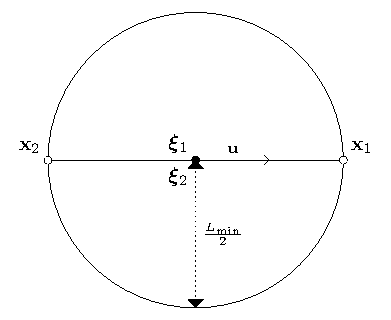
\includegraphics[]{figures/constraint_handling/well_length_zero.pdf}
	\caption{Minimum constraint violated. Initial points $\boldsymbol{\xi}_1, \boldsymbol{\xi}_2$ 
	are identical and solution points $\textbf{x}$ and $\textbf{y}$ lie on opposite sides of a circle 
	with radius $\frac{L_{\min}}{2}$. Note that the solution shown in the figure is only one of 
	the infinitely many solutions that exist for this case.}
	\label{fig:min_violation_zero}
\end{figure}
%
If $\| \boldsymbol{\xi}_1 - \boldsymbol{\xi}_2 \| < L_{\min}$ 
there are two solution types. If $\boldsymbol{\xi}_1 = \boldsymbol{\xi}_2$ 
then solutions are
%
\begin{equation}
\begin{aligned}
\textbf{x}_1 = \boldsymbol{\xi}_1 + \frac{L_{\min}}{2} \textbf{u}, \\
\textbf{x}_1 = \boldsymbol{\xi}_1 - \frac{L_{\min}}{2} \textbf{u},
\end{aligned}
\label{eq:solution_min_triv}
\end{equation}
%
for any vector $\textbf{u}$ of unit length. I.e., there is no unique solution and
all solutions are pairs of
points that lie on opposite sides of the circle with center $\boldsymbol{\xi}_1$ 
and radius $\frac{L_{\min}}{2}$. One such solution is shown in Figure
\ref{fig:min_violation_zero}.
%
\begin{figure}[H]
	\centering
	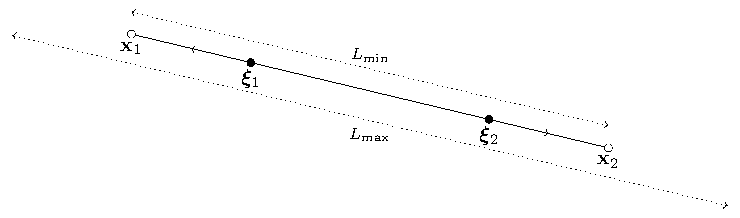
\includegraphics[]{figures/constraint_handling/well_length_min.pdf}
	\caption{Minimum constraint violated. Initial points $\boldsymbol{\xi}_1, \boldsymbol{\xi}_2$ 
	are too close and the solution is to move the points away from each other along the line that
	passes through them in opposite directions until the distance between them is exactly $L_{\min}$.}
	\label{fig:min_violation}
\end{figure}
%
If $\boldsymbol{\xi}_1 \neq \boldsymbol{\xi}_2$
then the solution is
%
\begin{equation}
\begin{aligned}
\textbf{x}_1 &= \boldsymbol{\xi}_1 + \frac{\lambda^*}{1 - 2\lambda^*} (\boldsymbol{\xi}_1 - \boldsymbol{\xi}_2), \\
\textbf{x}_2 &= \boldsymbol{\xi}_2 - \frac{\lambda^*}{1 - 2\lambda^*} (\boldsymbol{\xi}_1 - \boldsymbol{\xi}_2),
\end{aligned}
\label{eq:solution_min}
\end{equation}
were $ \lambda^* = \frac{1}{2} \left( 1 - \frac{\| \boldsymbol{\xi}_1 - \boldsymbol{\xi}_2 \|}{L_{\min}} \right)$.
Here both points are moved away from each other an equal distance along the line that passes through
$\boldsymbol{\xi}_1$ and $\boldsymbol{\xi}_2$ as shown in Figure \ref{fig:min_violation}.\\
%
%
\begin{figure}[H]
	\centering
	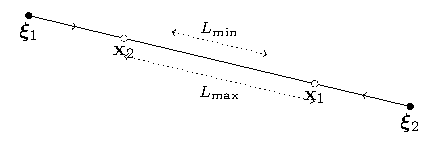
\includegraphics[]{figures/constraint_handling/well_length_max.pdf}
	\caption{Maximum constraint violated. Initial points $\boldsymbol{\xi}_1, \boldsymbol{\xi}_2$ 
	are too far away from each other and the solution is to move the points closer along the line 
	that passes through them until the distance between them is exactly $L_{\min}$.}
	\label{fig:max_violation}
\end{figure}
%
If $\| \boldsymbol{\xi}_1 - \boldsymbol{\xi}_2 \| > L_{\max}$
the solution is given by
\begin{equation}
\begin{aligned}
\textbf{x}_1 &= \boldsymbol{\xi}_1 - \frac{\mu^*}{1 + 2\mu^*} (\boldsymbol{\xi}_1 - \boldsymbol{\xi}_2), \\
\textbf{x}_2 &= \boldsymbol{\xi}_2 + \frac{\mu^*}{1 + 2\mu^*} (\boldsymbol{\xi}_1 - \boldsymbol{\xi}_2),
\end{aligned}
\label{eq:solution_max}
\end{equation}
where $\mu^* =\frac{1}{2} \left( \frac{\| \boldsymbol{\xi}_1 - \boldsymbol{\xi}_2 \|}{L_{\max}} - 1 \right) $. 
The geometric interpretation is that both points are moved closer to each other along the line that passes
through $\boldsymbol{\xi}_1$ and $\boldsymbol{\xi}_2$ as 
indicated in Figure \ref{fig:max_violation}.\\
%
\begin{figure}[H]
	\centering
	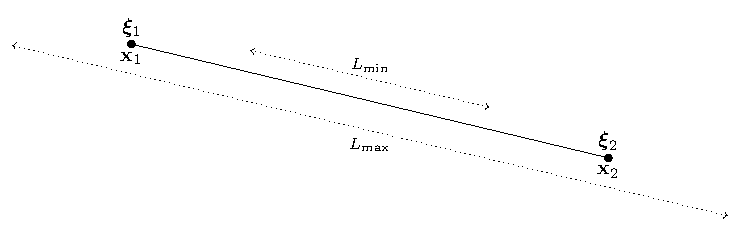
\includegraphics[]{figures/constraint_handling/well_length_feasible.pdf}
	\caption{Constraints are satisfied by initial points and no movement of the points is needed.}
	\label{fig:feasible}
\end{figure}
%
If $L_{\min} \leq \| \boldsymbol{\xi}_1 - \boldsymbol{\xi}_2 \| \leq L_{\max}$ the initial points
satisfy both constraints and as shown in 
Figure \ref{fig:feasible} we need not move them. 
The solution in this case is
\begin{equation}
\begin{aligned}
\textbf{x}_1 &= \boldsymbol{\xi}_1, \\
\textbf{x}_2 &= \boldsymbol{\xi}_2.
\label{eq:wl_formula_last}
\end{aligned}
\end{equation}
%
%
To prove the formulae \eqref{eq:solution_min_triv} -- \eqref{eq:wl_formula_last} 
consider the minimization problem \eqref{wlc_opt_1} -- \eqref{wlc_opt_3}, which can be 
solved by the method of Lagrange multipliers. Define the Lagrangian function
%
\begin{equation}
\begin{aligned}
\mathcal{L} (\textbf{x}_1,\textbf{x}_2,\lambda,\mu) &= \frac{1}{2} \| \textbf{x}_1 - \boldsymbol{\xi}_1 \|^2 + \frac{1}{2} \| \textbf{x}_2 - \boldsymbol{\xi}_2 \|^2 \\
&- \lambda \left( \frac{1}{2} \| \textbf{x}_1 - \textbf{x}_2 \|^2 - \frac{1}{2} L_{\min}^2 \right ) - \mu  \left( - \frac{1}{2} \| \textbf{x}_1 - \textbf{x}_2 \|^2 + \frac{1}{2} L_{\max}^2 \right ),
\end{aligned}
\label{lagrangeFunc}
\end{equation}
%
where $\lambda, \mu \in \mathbb{R}$ are the Lagrange multipliers for the constraints.
Note that only one of the constraints can be active at once, meaning that either $\lambda$
or $\mu$ must be zero.\\
A necessary condition for a local minimum $\textbf{x}_1^*, \textbf{x}_2^*$ is that 
it satisfies the first order KKT conditions
%
\begin{equation}
\begin{aligned}
\nabla_{\textbf{x}_1,\textbf{x}_2} \mathcal{L} (\textbf{x}_1^*, \textbf{x}_2^*, \lambda^*, \mu^*) &= 0, \\
\lambda h_1(\textbf{x}_1^*, \textbf{x}_2^*) &= 0,\\
\mu h_2(\textbf{x}_1^*, \textbf{x}_2^*) &= 0,\\
\lambda &\geq 0,\\
\mu &\geq 0,\\
h_i(\textbf{x}_1^*, \textbf{x}_2^*) &\geq 0, \qquad  i=1,2. \\
\end{aligned}
\end{equation}
%
Differentiating the Lagrangian and setting the gradient to 0 we obtain the system of equations
\begin{equation}
\begin{aligned}
\nabla_{\textbf{x}_1} \mathcal{L} &= \textbf{x}_1 - \boldsymbol{\xi}_1 - \lambda ( \textbf{x}_1 - \textbf{x}_2 ) + \mu ( \textbf{x}_1 - \textbf{x}_2 ) = 0, \\
\nabla_{\textbf{x}_2} \mathcal{L} &= \textbf{x}_2 - \boldsymbol{\xi}_2 + \lambda ( \textbf{x}_1 - \textbf{x}_2 ) - \mu ( \textbf{x}_1 - \textbf{x}_2 ) = 0. \\
\end{aligned}
\label{eq:gradients}
\end{equation}
%
%
The problem is solved by dividing the positions of the initial points, $\boldsymbol{\xi}_1 $ 
and $\boldsymbol{\xi}_2$ into three different cases and then considering different candidate 
solutions $(\textbf{x}_1^*, \textbf{x}_2^*, \lambda^*, \mu^*)$. The three different categories
for the initial position of the heel and toe of the well must either violate exactly one of the
constraints, or violate none of them. The optimal solution of a configuration must satisfy the
constraints, i.e., $L_{\min} \leq \| \textbf{x}_1^* - \textbf{x}_2^* \| \leq L_{\max}$. A solution
must satisfy exactly one of the following equations
%
\begin{equation}
\begin{aligned}
L_{\min} < \| \textbf{x}_1^* - \textbf{x}_2^* \| &< L_{\max}, \\
\| \textbf{x}_1^* - \textbf{x}_2^* \| &= L_{\min}, \\
\| \textbf{x}_1^* - \textbf{x}_2^* \| &= L_{\max}.
\label{eq:intercategories}
\end{aligned}
\end{equation}
%
For each of the three cases for the initial positions of the well we will
consider each of the three possibilities for the solution.
%
\subsection{Case 1. Initial points feasible}
%
Assume that $ L_{\min} \leq \| \boldsymbol{\xi}_1 - \boldsymbol{\xi}_2 \| \leq L_{\max} $.
Then the initial points satisfy the distance constraint and no movement of the points is needed. 
Because the objective function $f$ is non-negative
and $f(\boldsymbol{\xi}_1,\boldsymbol{\xi}_2) = 0$ this solution is the global minimum.
%
%
\subsection{Case 2. Initial points too close}
%
Assume that $ \| \boldsymbol{\xi}_1 - \boldsymbol{\xi}_2 \| < L_{\min} $.
The distance between the initial points is too small and must be increased.
%
According to \eqref{eq:intercategories} there are three different possibilities 
for the distance between the candidate solutions $\textbf{x}_1^*, \textbf{x}_2^*$. 
%
If 
\begin{equation}
L_{\max} >  \| \textbf{x}_1^* - \textbf{x}_2^*  \| > L_{\min},
\label{eq:interior}
\end{equation}
i.e., the solution lies in the interior of both constraints. 
Then none of the constraints are active, which gives
$\lambda^* =\mu^* = 0 $ and therefore
%
\begin{equation}
\begin{aligned}
    	\textbf{x}_1^* &= \boldsymbol{\xi}_1,\\
    	\textbf{x}_2^* &= \boldsymbol{\xi}_2.
\end{aligned}
\end{equation}
%
But this results in the contradiction 
$\| \textbf{x}_1^* - \textbf{x}_2^*  \| = \| \boldsymbol{\xi}_1 - \boldsymbol{\xi}_2 \| \leq L_{\min},$ 
and thus the solution cannot satisfy \eqref{eq:interior}.\\
%
%
If $\| \textbf{x}_1^* - \textbf{x}_2^*  \| = L_{\min}$, the maximum
constraint is inactive which means that $\mu = 0$. Inserting this into 
equation \eqref{eq:gradients} gives
%
\begin{equation}
\begin{aligned}
\textbf{x}_1 - \boldsymbol{\xi}_1 - \lambda ( \textbf{x}_1 - \textbf{x}_2 )  &= 0, \\
\textbf{x}_2 - \boldsymbol{\xi}_2 + \lambda ( \textbf{x}_1 - \textbf{x}_2 )  &= 0,
\end{aligned}
\label{eq:gradients_2.1}
\end{equation}
%
which is a linear system with respect to $\textbf{x}_1$ and $\textbf{x}_2$.
Now if $\boldsymbol{\xi}_1 = \boldsymbol{\xi}_2$, which means the initial well has zero length,
then it follows that $\lambda=\frac{1}{2}$ and we get
%
\begin{align}
\textbf{x}_1 + \textbf{x}_2 &= 2 \boldsymbol{\xi}_1, \\
\| \textbf{x}_1^* - \textbf{x}_2^*\| &= L_{\min}.
\label{eq:zero_length_solution}
\end{align}
%
This equation has solutions
\begin{align}
\textbf{x}_1 = \boldsymbol{\xi}_1 + \frac{L_{\min}}{2} \textbf{u} , \\
\textbf{x}_1 = \boldsymbol{\xi}_1 - \frac{L_{\min}}{2} \textbf{u} ,
\label{eq:zero_length_solutions}
\end{align}
for all unit vectors $\textbf{u}$ and they are all KKT points. So if the initial 
well has zero length the solutions all lie on a circle with center $\boldsymbol{\xi}_2$ 
and radius $\frac{L_{\min}}{2}$.
%
Now if $\boldsymbol{\xi}_1 \neq \boldsymbol{\xi}_2$, then 
solving the system \eqref{eq:gradients_2.1} gives
%
\begin{equation}
\begin{aligned}
\textbf{x}_1 &=  \frac{1}{(1-\lambda)^2 -(\lambda)^2 } \left( (1-\lambda) \boldsymbol{\xi}_1 - \lambda \boldsymbol{\xi}_2 \right) 
= \boldsymbol{\xi}_1 + \frac{\lambda}{1 - 2\lambda} (\boldsymbol{\xi}_1 - \boldsymbol{\xi}_2), \\
\textbf{x}_2 &=  \frac{1}{(1-\lambda)^2 -(\lambda)^2 } \left(-\lambda \boldsymbol{\xi}_1 + (1-\lambda) \boldsymbol{\xi}_2 \right)
= \boldsymbol{\xi}_2 - \frac{\lambda}{1 - 2\lambda} (\boldsymbol{\xi}_1 - \boldsymbol{\xi}_2).
\end{aligned}
\label{eq:solutions_2.2}
\end{equation}
%
Combining this result with the condition that $\| \textbf{x}_1^* - \textbf{x}_2^*\| = L_{\min}$ we obtain
%
\begin{equation}
\lambda^* = \frac{1}{2} \left( 1 \pm \frac{\| \boldsymbol{\xi}_1 - \boldsymbol{\xi}_2 \|}{L_{\min}} \right),
\label{eq:solutions_lambda_2.2}
\end{equation}
%
where both candidates for $\lambda^*$ are positive and therefore yield KKT points.
From \eqref{eq:gradients_2.1} we have
%
\begin{equation}
f(\textbf{x}_1,\textbf{x}_2) = \lambda^2 \| \textbf{x}_1 - \textbf{x}_2\|^2,
\label{eq:well_length_min}
\end{equation}
%
and thus the minimum is attained for the smaller candidate. The best KKT point is therefore given by

\begin{equation}
\begin{aligned}
\textbf{x}_1^* &= \boldsymbol{\xi}_1 + \frac{\lambda^*}{1 - 2\lambda^*} (\boldsymbol{\xi}_1 - \boldsymbol{\xi}_2), \\
\textbf{x}_2^* &= \boldsymbol{\xi}_2 - \frac{\lambda^*}{1 - 2\lambda^*} (\boldsymbol{\xi}_1 - \boldsymbol{\xi}_2),
\label{eq:best_min}
\end{aligned}
\end{equation}
where 
$\lambda^* = \frac{1}{2} \left( 1 - \frac{\| \boldsymbol{\xi}_1 - \boldsymbol{\xi}_2 \|}{L_{\min}} \right).$
%
%

The last possibility is that $L_{\max} =  \| \textbf{x}_1^* - \textbf{x}_2^*  \|$.
%
The derivation is similar to the previous case.
The maximum constraint is active so therefore the other
constraint is inactive and hence $\lambda = 0.$
If $\boldsymbol{\xi}_1 = \boldsymbol{\xi}_2$ then we get infinitely 
many solutions
%
\begin{align}
\textbf{x}_1 + \textbf{x}_2 &= 2 \boldsymbol{\xi}_1, \\
\| \textbf{x}_1^* - \textbf{x}_2^*\| &= L_{\max},
\label{eq:zero_length_solution_max}
\end{align}
%
but since these all lie on a circle with center in $\boldsymbol{\xi}_1$ and radius
$\frac{L_{\max}}{2}$ the solutions are all worse than the ones in \eqref{eq:zero_length_solutions}
so none of them can be a global minimum.
%
\begin{equation}
\begin{aligned}
\textbf{x}_1 =  \frac{1}{(1+\mu)^2 -(\mu)^2 } \left( (1+\mu) \boldsymbol{\xi}_1 + \mu \boldsymbol{\xi}_2 \right) 
= \boldsymbol{\xi}_1 - \frac{\mu}{1+2 \mu} (\boldsymbol{\xi}_1 - \boldsymbol{\xi}_2), \\
\textbf{x}_2 =  \frac{1}{(1+\mu)^2 -(\mu)^2 } \left( \mu \boldsymbol{\xi}_1 + (1+\mu) \boldsymbol{\xi}_2 \right)
= \boldsymbol{\xi}_2 + \frac{\mu}{1+2 \mu} (\boldsymbol{\xi}_1 - \boldsymbol{\xi}_2).
\end{aligned}
\label{eq:solutions_2.3}
\end{equation}
%
Using the fact that $L_{\max} =  \| \textbf{x}_1^* - \textbf{x}_2^*  \|$ 
and solving for $\mu$ results in
%
\begin{equation}
\mu = - \frac{1}{2} \left( 1 \pm \frac{\| \boldsymbol{\xi}_1 - \boldsymbol{\xi}_2 \|}{L_{\max}} \right) < 0,
\label{eq:solutions_mu_2.3}
\end{equation}
%
which are not solutions since the Lagrange multiplier in both cases is negative.
Now it follows that, since there are only two points that satisfy the KKT
conditions, the better one has to be the global optimum, and thus the
solution for Case 2 is given by \eqref{eq:best_min}
%
%
\subsection{Case 3. Initial points too distant}
%
The initial condition is that $ \| \boldsymbol{\xi}_1 - \boldsymbol{\xi}_2 \| > L_{\max}$,
which means that the initial points are too far away from each other and need to
be moved closer to each other.
The solutions for this case are analogous to Case 2 and the calculations 
will be omitted. The only valid solution is found when
$\| \textbf{x}_1^* - \textbf{x}_2^*  \| = L_{\max}$ which results in
$\mu^* = \frac{1}{2} \left( - 1 + \frac{\| \boldsymbol{\xi}_1 - \boldsymbol{\xi}_2 \|}{L_{\max}} \right)$
and $\lambda^* = 0$. This gives the solution 
\begin{equation}
\begin{aligned}
\textbf{x}_1^* &= \boldsymbol{\xi}_1 - \frac{\mu^*}{1 + 2\mu^*} (\boldsymbol{\xi}_1 - \boldsymbol{\xi}_2), \\
\textbf{x}_2^* &= \boldsymbol{\xi}_2 + \frac{\mu^*}{1 + 2\mu^*} (\boldsymbol{\xi}_1 - \boldsymbol{\xi}_2).
\end{aligned}
\end{equation}

%
%
%
% ██╗███╗   ██╗████████╗███████╗██████╗     ██╗    ██╗███████╗██╗     ██╗         ██████╗ ██╗███████╗████████╗ █████╗ ███╗   ██╗ ██████╗███████╗
% ██║████╗  ██║╚══██╔══╝██╔════╝██╔══██╗    ██║    ██║██╔════╝██║     ██║         ██╔══██╗██║██╔════╝╚══██╔══╝██╔══██╗████╗  ██║██╔════╝██╔════╝
% ██║██╔██╗ ██║   ██║   █████╗  ██████╔╝    ██║ █╗ ██║█████╗  ██║     ██║         ██║  ██║██║███████╗   ██║   ███████║██╔██╗ ██║██║     █████╗  
% ██║██║╚██╗██║   ██║   ██╔══╝  ██╔══██╗    ██║███╗██║██╔══╝  ██║     ██║         ██║  ██║██║╚════██║   ██║   ██╔══██║██║╚██╗██║██║     ██╔══╝  
% ██║██║ ╚████║   ██║   ███████╗██║  ██║    ╚███╔███╔╝███████╗███████╗███████╗    ██████╔╝██║███████║   ██║   ██║  ██║██║ ╚████║╚██████╗███████╗
% ╚═╝╚═╝  ╚═══╝   ╚═╝   ╚══════╝╚═╝  ╚═╝     ╚══╝╚══╝ ╚══════╝╚══════╝╚══════╝    ╚═════╝ ╚═╝╚══════╝   ╚═╝   ╚═╝  ╚═╝╚═╝  ╚═══╝ ╚═════╝╚══════╝
\section{Inter-well distance constraint}
%
Minimize the movement of the endpoints of two line 
segments such that every point on the first 
line segment is at least some distance $d$ away 
from every point on the other line segment.
%
Let the initial positions of the two line segments be 
defined by their endpoints 
$\boldsymbol{\xi}_1, \boldsymbol{\xi}_2, \boldsymbol{\xi}_3, \boldsymbol{\xi}_4 \in \mathbb{R}^3$ 
respectively. Minimizing the movement is the solution to the problem
%
\begin{equation}
\min_{ \textbf{x}_i \in \mathbb{R}^3 } F(\textbf{x}_1,\textbf{x}_2,\textbf{x}_3,\textbf{x}_4) = \min_{ \textbf{x}_i \in \mathbb{R}^3 } \sum_{i=1}^4 \frac{1}{2} \| \textbf{x}_i - \boldsymbol{\xi}_i \|^2
\label{eq:interwell_distance}
\end{equation}
under the conditions that
\begin{align}
c(\textbf{x}_1,\textbf{x}_2,\textbf{x}_3,\textbf{x}_4,\lambda_1,\lambda_2) \geq \frac{1}{2} d^2\label{eq:interwell_distance_constraint}\\
\intertext{for all} 
\quad \lambda_i \in [0,1], \quad i=1,2,	\label{eq:interwell_distance_lambda}
\end{align}
%
where
%
\begin{equation}
c(\textbf{x}_1,\textbf{x}_2,\textbf{x}_3,\textbf{x}_4,\lambda_1,\lambda_2) = 
\frac{1}{2} \| (\textbf{x}_1 + \lambda_1 (\textbf{x}_2 - \textbf{x}_1 )) - (\textbf{x}_3 + \lambda_2 (\textbf{x}_4 - \textbf{x}_3)) \|^2.
\end{equation}
%
Call a solution in which $k$ points are moved a $k$-point solution. We will first
try to solve \eqref{eq:interwell_distance} -- \eqref{eq:interwell_distance_lambda} by
moving only two points, then by moving just three points, and lastly, if a solution is
not yet found, move all four points. The idea is that, if the optimal solution for
moving two or three points while temporarily ignoring the other point(s) satisfies all
the constraints in \eqref{eq:interwell_distance_lambda}, then this must be the 
optimal solution to \eqref{eq:interwell_distance}. \\
%
To see why this is true, notice that in general if $\Omega_1 \subset \Omega_2$,
then
\begin{align}
\min_{x \in \Omega_1} f(x) \geq \min_{x \in \Omega_2} f(x)
\label{eq:set_min}
\end{align}
holds for all real valued functions $f$. Thus if we have that
%
\begin{align}
 f(x^*) = \min_{x \in \Omega_2} f(x) \quad \text{and} \quad x^* \in \Omega_1,
\end{align}
%
then $x^*$ is feasible for the first problem and 
%
\begin{align}
f(x^*) \leq f(x) \quad \forall x \in \Omega_1,
\end{align}
%
which means that $x^*$ is the solution to both minimization problems, i.e.,
%
\begin{align}
\min_{x \in \Omega_1} f(x) = \min_{x \in \Omega_2} f(x) = f(x^*).
\label{eq:set_min_end}
\end{align}
% 
Now ignoring one of the four points is the same as setting either $\lambda_1$ or
$\lambda_2$ equal to 1 or 0 in \eqref{eq:interwell_distance_lambda}. E.g., if we
wish to only consider the points $\textbf{x}_1, \textbf{x}_2$ and $\textbf{x}_4$
but ignore $\textbf{x}_3$ this is done by letting $\lambda_2 = 1$. Call the set
of feasible points for a $k$-point problem $\tilde{\Omega}_k$. Clearly we must
have $\tilde{\Omega}_4 \subset \tilde{\Omega}_3 \subset \tilde{\Omega}_2 \subset \tilde{\Omega}_1$. Then by 
\eqref{eq:set_min} -- \eqref{eq:set_min_end} we have that the $k$-point solution 
with the smallest value for $k$ which is feasible in the four point problem, 
must also be the solution to the four point problem.

%
\subsection[Number of points moved]{Number of points moved and form of solutions}
%
A line segment that connects the two solution line segments, $S_1, S_2$, over the 
shortest distance will be called SD (Shortest Distance). If only one of the two line 
segments is needed in a figure then, without loss of generality, we will refer to this
line segment as $S_1$ with endpoints $\textbf{x}_1$ and $\textbf{x}_2$. Divide the solutions of the
problem into different categories depending on how many of the points have been moved. 
Denote the smallest angle between the SD and $S_i$ by $\alpha_i$. Note that SD is not
unique if $S_1$ and $S_2$ are parallel, but the angles $\alpha_1$ and $\alpha_2$ are.
We must also have that $\alpha_i \geq 90^\circ$. If one angle is below $90^\circ$ then there 
exists a shorter distance between the line segments by moving the SD along 
the line segment in the direction of the angle as indicated by the arrow
in Figure \ref{fig:four_point_all_alpha}. 
%
\begin{figure}[H]
	\centering
	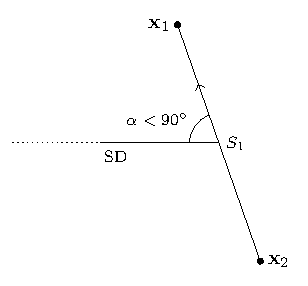
\includegraphics[width=0.45\textwidth]{figures/constraint_handling/interwell_angles.pdf}
	\caption{Candidate for shortest distance (SD). A shorter distance between the segments
			 can be found by moving upwards along the line segment.}
	\label{fig:four_point_all_alpha}
\end{figure}
%
%
If one angle $\alpha$ is over 90 degrees, then the SD must connect to an endpoint
of the corresponding line segment (or else SD could be improved by moving it along the line
segment) as shown in Figure \ref{fig:four_point_angles_4p}. 
%
\begin{figure}[H]
	\centering
	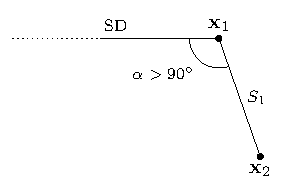
\includegraphics[width=0.45\textwidth]{figures/constraint_handling/interwell_angles_4p.pdf}
	\caption{One angle over 90 degrees. Moving $\textbf{x}_2$ does not change the length of SD.}
	\label{fig:four_point_angles_4p}
\end{figure}
%
Assume that this is the case.
Without loss of generality we call this endpoint $\textbf{x}_1$ and the other endpoint of
the line segment $\textbf{x}_2$. Then moving $\textbf{x}_2$ a small distance does not
change the shortest distance. It follows that $\textbf{x}_2 = \boldsymbol{\xi}_2$ because
no constraints are active for $\textbf{x}_2$ and this cannot be a solution where all four
points have been moved. Therefore, in a solution where all four points are moved,
both of the angles must be 90 degrees.
%
If we have a case where both angles are over 90 degrees as shown in
Figure \ref{fig:four_point_angles_3p}, then the SD connects two
endpoints,
%
\begin{figure}[H]
	\centering
	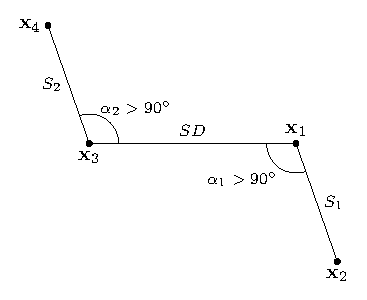
\includegraphics[width=0.45\textwidth]{figures/constraint_handling/interwell_angles_3p.pdf}
	\caption{One angle over 90 degrees}
	\label{fig:four_point_angles_3p}
\end{figure}
%
\noindent and by applying the same argument as above to 
both line segments we see this is a solution where at most
two points have been moved. Thus it cannot be a three-point solution.
Therefore a three-point solution must have one angle $\alpha$
equal to $90^{\circ}$ and the other one larger than $90^{\circ}$.
%
If we are left with both angles larger than $90^{\circ}$ then we must have moved either
two points or no points.
%
\subsection{Four-point solution}
%
Denote the initial points $\boldsymbol{\xi}_1, \boldsymbol{\xi}_2, \boldsymbol{\xi}_3$ 
and $\boldsymbol{\xi}_4$ and the solution points $\textbf{x}_1, \textbf{x}_2, \textbf{x}_3$ 
and $\textbf{x}_4$. In the solution the SD will be orthogonal to both line segments. 
This means that in the solution the line segments will lie in two planes $E^1$ and $E^2$
that share the same normal vector (namely SD). This means that $E^1$ and $E^2$ are parallel 
and a distance $d$ apart. 
Let
%
\begin{equation}
E^0 = E_{\textbf{s},t} = \{ \textbf{x} : \langle \textbf{s},\textbf{x} \rangle = t \}
\end{equation} 
be the plane that lies between the two solution planes with $\textbf{s}$ the
normalized SD vector (pointing towards the line segment with endpoints $\textbf{x}_1, \textbf{x}_2$)
and $t \in \mathbb{R}$.
%
\begin{figure}[H]
	\centering
	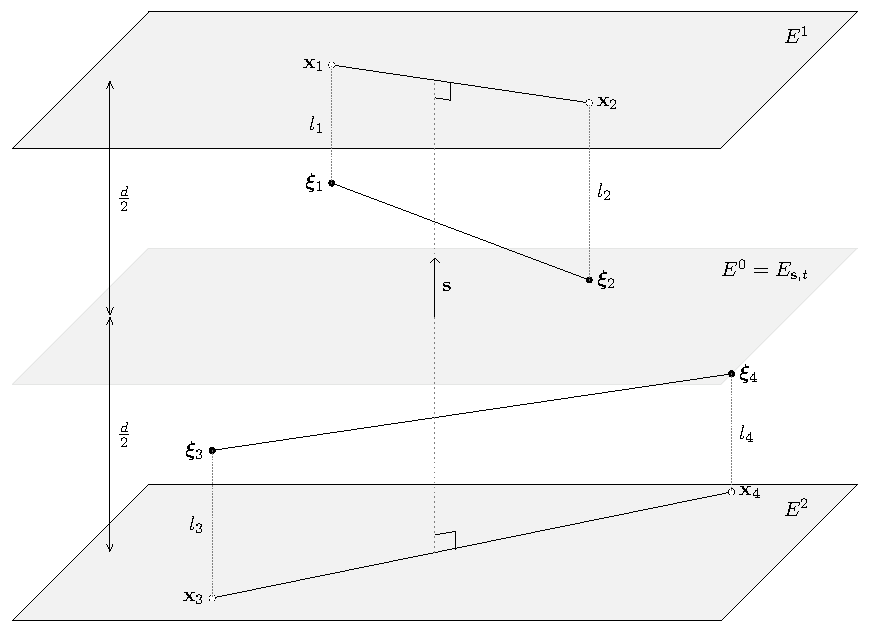
\includegraphics[width=0.95\textwidth]{figures/constraint_handling/four_point_interwell_problem.pdf}
	\caption{Four point solution. All four initial points have been moved and the resulting shortest distance
			 line is orthogonal to both solutions. Project initial points down on planes to get the optimal
			 solution.}
	\label{fig:four_point_problem}
\end{figure}
%
If the two planes $E^1$ and $E^2$ are found, then the solution is simply
the shortest distance from the initial points to the planes, which is found by projecting 
$\textbf{x}_1$ and $\textbf{x}_2$ onto $E^1 = E_{\textbf{s},t+\frac{d}{2}}$ and by projecting
$\textbf{x}_3$ and $\textbf{x}_4$ onto $E^2 = E_{\textbf{s},t-\frac{d}{2}}$.
%
Denote
%
\begin{equation}
\begin{aligned}
l_1(\textbf{s},t) &=  \langle \textbf{s}, \boldsymbol{\xi}_1 \rangle - t  - \frac{d}{2}, \\
l_2(\textbf{s},t) &=  \langle \textbf{s}, \boldsymbol{\xi}_2 \rangle - t  - \frac{d}{2}, \\
l_3(\textbf{s},t) &=  \langle \textbf{s}, \boldsymbol{\xi}_3 \rangle - t  + \frac{d}{2}, \\
l_4(\textbf{s},t) &=  \langle \textbf{s}, \boldsymbol{\xi}_4 \rangle - t  + \frac{d}{2},
\label{eq:interwell_lengths} 
\end{aligned}
\end{equation}
%
then $|l_i(\textbf{s},t)| = \| \textbf{x}_i - \boldsymbol{\xi}_i \|$.
Thus we can rewrite the minimization problem \eqref{eq:interwell_distance} 
and solve for $\textbf{s}$ and $t$ by
%
\begin{equation}
\min_{ \textbf{x}_i \in \mathbb{R}^3 } F(\textbf{x}_1,\textbf{x}_2,\textbf{x}_3,\textbf{x}_4) 
= \min_{ \textbf{s} \in \mathbb{S}^2, t \in \mathbb{R}} \frac{1}{2}  \sum_{i=1}^4 l_i(\textbf{s},t)^2.
\label{eq:interwell_st}
\end{equation}
%
Holding $\textbf{s}$ fixed and minimizing $F$ with respect to $t$ gives
the condition
%
\begin{align}
\frac{\partial F}{\partial t} (\textbf{s},t) =  
   &\langle \textbf{s},\boldsymbol{\xi}_1 \rangle - t  - \frac{d}{2} 
+  \langle \textbf{s},\boldsymbol{\xi}_2 \rangle - t  - \frac{d}{2} \\
&+ \langle \textbf{s},\boldsymbol{\xi}_3 \rangle - t  + \frac{d}{2} 
+  \langle \textbf{s},\boldsymbol{\xi}_4 \rangle - t  + \frac{d}{2} \\
= &\sum_{i=1}^4 \langle \boldsymbol{\xi}_i,\textbf{s} \rangle - 4t = 0, \\
\intertext{and therefore} 
t = &\frac{1}{4} \sum_{i=1}^4 \langle \boldsymbol{\xi}_i,\textbf{s} \rangle.
\end{align}
%
We simplify the problem by introducing the shifted variables
\begin{equation}
\hat{\boldsymbol{\xi}}_i = \boldsymbol{\xi}_i - \frac{1}{4} \sum_{i=1}^4 \boldsymbol{\xi}_i.
\end{equation}
%
We then get the identity
%
\begin{equation}
\begin{aligned}
\langle \textbf{s},\boldsymbol{\xi}_i \rangle   &= \langle \textbf{s},\hat{\boldsymbol{\xi}}_i \rangle
												+  \langle \textbf{s},\boldsymbol{\xi}_i - \hat{\boldsymbol{\xi}}_i \rangle\\
										        &= \langle \textbf{s},\hat{\boldsymbol{\xi}}_i \rangle 
										       	+  \Big\langle \textbf{s}, \frac{1}{4} \sum_{i=1}^4 \boldsymbol{\xi}_i \Big\rangle\\
												&= \langle \textbf{s},\hat{\boldsymbol{\xi}}_i \rangle
												+  \frac{1}{4} \sum_{i=1}^4 \langle \textbf{s},\boldsymbol{\xi}_i \rangle.
\end{aligned}												  
\end{equation}
%
For the shifted variables inserted into \eqref{eq:interwell_lengths} 
the variable $t$ is eliminated and equation \eqref{eq:interwell_st} 
can be rewritten as
%
\begin{equation}
\min_{ \textbf{s} \in \mathbb{S}^2, t \in \mathbb{R}} F(\textbf{s},t)=\min_{ \textbf{s} \in \mathbb{S}^2} \frac{1}{2}  \sum_{i=1}^4 \hat{l}_i(\textbf{s})^2
\end{equation}
%
with
%
\begin{equation}
\begin{aligned}
\hat{l}_1(\textbf{s},t) &=  \langle \textbf{s},\hat{\boldsymbol{\xi}}_1 \rangle - \frac{d}{2}, \\
\hat{l}_2(\textbf{s},t) &=  \langle \textbf{s},\hat{\boldsymbol{\xi}}_2 \rangle - \frac{d}{2}, \\
\hat{l}_3(\textbf{s},t) &=  \langle \textbf{s},\hat{\boldsymbol{\xi}}_3 \rangle + \frac{d}{2}, \\
\hat{l}_4(\textbf{s},t) &=  \langle \textbf{s},\hat{\boldsymbol{\xi}}_4 \rangle + \frac{d}{2}.
\label{eq:interwell_lengths_trans} 
\end{aligned}
\end{equation}
%
We differentiate $F$ with respect to $\textbf{s}$ to get
%
\begin{equation}
\frac{\partial F}{\partial \textbf{s}} (\textbf{s}) =  \sum_{i=1}^4 (\hat{\boldsymbol{\xi}}_i \otimes \hat{\boldsymbol{\xi}}_i)\textbf{s}
- \frac{d}{2}(\hat{\boldsymbol{\xi}}_1 + \hat{\boldsymbol{\xi}}_2) + \frac{d}{2}(\hat{\boldsymbol{\xi}}_3 + \hat{\boldsymbol{\xi}}_4).
\end{equation}
%
Let
%
\begin{equation}
A = \sum_{i=1}^4 \hat{\boldsymbol{\xi}}_i \otimes \hat{\boldsymbol{\xi}}_i \quad \text{and} \quad 
b = \frac{d}{2}(\hat{\boldsymbol{\xi}}_1 + \hat{\boldsymbol{\xi}}_2 - \hat{\boldsymbol{\xi}}_3 - \hat{\boldsymbol{\xi}}_4).
\label{eq:A_b_four_points}
\end{equation}
%
With the constraint $\| \textbf{s}\|^2 = 1$
we get the necessary KKT conditions
%
\begin{equation}
\begin{aligned}
(A-\mu I)\textbf{s} &= b,\\
\|\textbf{s}\|^2 &= 1,
\label{eq:interwell_matrix}
\end{aligned}
\end{equation}
%
where $\mu \in \mathbb{R}$ is a Lagrange parameter.
%
Either $\mu$ is an eigenvalue
of $A$, or $A-\mu I$ is invertible.
%
Assume first that $\mu$ is not an eigenvalue of $A$. This means that
$A-\mu I$ is invertible and we can write
%
\begin{align}
\textbf{s} = (A-\mu I)^{-1}b.
\end{align}
%
Since $A$ is symmetric it can be diagonalized and written as $A = QDQ^T$ with
orthogonal matrix $Q$ and a diagonal matrix $D$ containing the eigenvalues of $A$. 
Inserting this into \eqref{eq:interwell_matrix} gives
%
\begin{equation}
\textbf{s} = (A-\mu I)^{-1}b = Q(D-\mu I)^{-1}Q^Tb.
\label{eq:interwell_s}
\end{equation}
%
Take the norm (orthogonal matrices do not change the norm of a vector) of both sides to get
%
\begin{equation}
\| (D-\mu I)^{-1}Q^Tb \|^2= 1,
\end{equation}
%
or equivalently 
%
\begin{equation}
\sum_{i=1}^3 \frac{1}{(D_i-\mu)^2} (Q^Tb)_i^2 = 1.
\label{eq:six_degree_poly}
\end{equation}
%
The result is a sixth degree equation in $\mu$ which can have up to six distinct solutions,
all of which satisfy the KKT conditions.\\
%
If $\mu$ is an eigenvalue of $A$ then $A-\mu I$ is not
invertible and
%
\begin{align}
(A-\mu I)\textbf{s} &= b
\label{eq:non_invertible_interwell}
\end{align}
%
has either no solutions or infinitely many solutions. If solutions exist 
assume that $\textbf{s}_0$ solves \eqref{eq:non_invertible_interwell}. Then
$\ker(A-\mu I) + \textbf{s}_0$ is the space of all solutions to \eqref{eq:non_invertible_interwell}.
%
So if there exists solutions to \eqref{eq:non_invertible_interwell} we
only need to find a single solution $\textbf{s}_0$ and $\ker(A-\mu I)$.
By requiring that
%
\begin{align}
\| \textbf{s} \|^2 = 1,
\end{align}
%
we obtain that the solutions space is the intersection of $\mathbb{S}^2$ with either
a line, a plane or $\mathbb{R}^3$. The solution space depends on the multiplicity of
the eigenvalues of $(A-\mu I)$ and the vector $b$.
%
%
All solutions for $\mu$ are KKT points, but they need not all be local minima. 
The vector $\textbf{s}$ is found by substituting $\mu$ back into equation 
\eqref{eq:interwell_s}, and then the best solution can be found by projecting 
the initial points to the planes as shown in Figure \ref{fig:four_point_problem} and 
comparing different values of $F$ for each configuration.
%
%
%
\subsection{Three-point solution}
Assume that the initial coordinate $\boldsymbol{\xi}_1$ belongs to line segment $S_1$
and that the coordinates $\boldsymbol{\xi}_2$ and $\boldsymbol{\xi}_2$ belong to the
other line segment $S_2$.
In the solution the SD will start in $\textbf{x}_1$ and be orthogonal to the line
segment defined by $\textbf{x}_2$ and $\textbf{x}_3$. The solution for this case is 
analogous to the four point case. Again we have the two planes $E^1$ and $E^2$, 
and we also have that $\textbf{x}_1 \in E^1$ and $\textbf{x}_2, \textbf{x}_3 \in E^2$ as shown in 
Figure \ref{fig:three_point_problem}.
%
\begin{figure}[H]
	\centering
	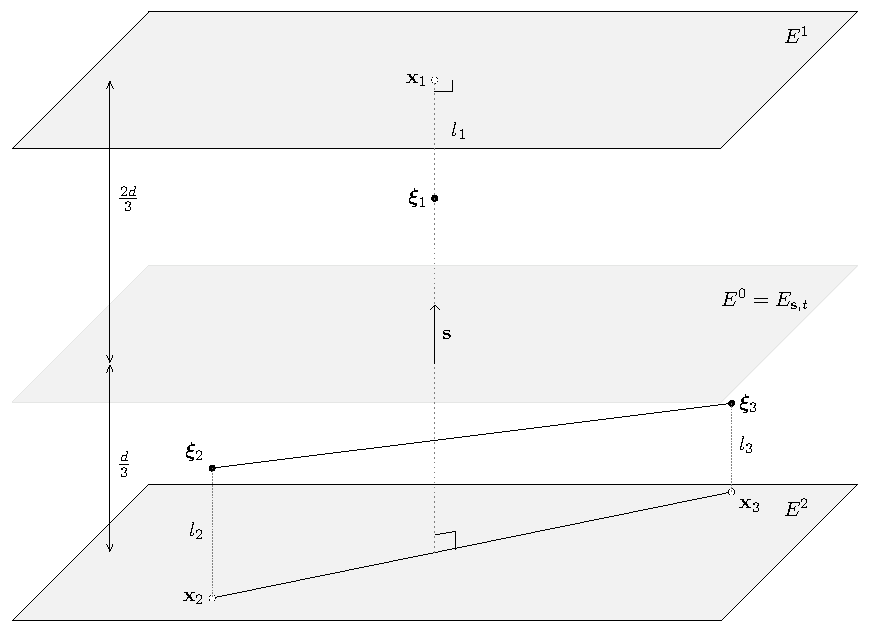
\includegraphics[width=0.95\textwidth]{figures/constraint_handling/three_point_interwell_problem.pdf}
	\caption{Three point problem}
	\label{fig:three_point_problem}
\end{figure}
%
We solve
\begin{align}
\min_{ \textbf{s} \in \mathbb{S}^2, t \in \mathbb{R}} F(\textbf{s},t) = \min_{ \textbf{s} \in \mathbb{S}^2, t \in \mathbb{R}}  \frac{1}{2} \sum_{i=1}^3 l_i(\textbf{s},t)^2,
\label{interwell_3point_problem}
\end{align}

where the lengths of the projections, $l_i$, are given by
%
\begin{align}
l_1(\textbf{s},t) &=  \langle \textbf{s}, \boldsymbol{\xi}_1 \rangle - t  - \frac{2d}{3}, \\
l_2(\textbf{s},t) &=  \langle \textbf{s}, \boldsymbol{\xi}_2 \rangle - t  + \frac{d}{3}, \\
l_3(\textbf{s},t) &=  \langle \textbf{s}, \boldsymbol{\xi}_3 \rangle - t  + \frac{d}{3}.
\label{eq:interwell_lengths_3p}
\end{align}
%
Again we minimize $F$ with respect to $t$ to get
\begin{align}
t &= \frac{1}{3} \sum_{i=1}^3 \langle \boldsymbol{\xi}_i,\textbf{s} \rangle.
\label{eq:three_point_t}
\end{align} 
Introducing the shifted variables
\begin{equation}
\hat{\boldsymbol{\xi}}_i = \boldsymbol{\xi}_i - \frac{1}{3} \sum_{i=1}^3 \boldsymbol{\xi}_i
\end{equation}
and using the value for $t$ found in \eqref{eq:three_point_t} and inserting these into
\eqref{interwell_3point_problem} we obtain the simplified problem
%
\begin{align}
\min_{ \textbf{s} \in \mathbb{S}^2, t \in \mathbb{R}} F(\textbf{s},t) = \min_{ \textbf{s} \in \mathbb{S}^2} \frac{1}{2} \sum_{i=1}^3 \hat{l}_i(\textbf{s})^2,
\label{interwell_3point_problem_shifted}
\end{align}
%
where 
%
\begin{align}
\hat{l}_1(\textbf{s},t) &=  \langle \textbf{s}, \hat{\boldsymbol{\xi}}_1 \rangle - \frac{2d}{3}, \\
\hat{l}_2(\textbf{s},t) &=  \langle \textbf{s}, \hat{\boldsymbol{\xi}}_2 \rangle + \frac{d}{3}, \\
\hat{l}_3(\textbf{s},t) &=  \langle \textbf{s}, \hat{\boldsymbol{\xi}}_3 \rangle + \frac{d}{3}.
\label{eq:interwell_lengths_3p_shifted}
\end{align}
%
We differentiate $F$ with respect to $\textbf{s}$ which gives
%
\begin{equation}
\frac{\partial F}{\partial \textbf{s}} (\textbf{s}) =  \sum_{i=1}^3 (\hat{\boldsymbol{\xi}}_i \otimes \hat{\boldsymbol{\xi}}_i)\textbf{s}
- \frac{2d}{3}\hat{\boldsymbol{\xi}}_1 + \frac{d}{3}(\hat{\boldsymbol{\xi}}_2 + \hat{\boldsymbol{\xi}}_3).
\end{equation}
%
A vector $\textbf{s}$ vector satisfies the necessary KKT conditions if it solves \eqref{eq:interwell_matrix} with
%
\begin{equation}
A = \sum_{i=1}^3 \hat{\boldsymbol{\xi}}_i \otimes \hat{\boldsymbol{\xi}}_i \quad \text{and} \quad 
b = \frac{2d}{3}\hat{\boldsymbol{\xi}}_1 - \frac{d}{3}(\hat{\boldsymbol{\xi}}_2 - \hat{\boldsymbol{\xi}}_3).
\label{eq:A_b_three_points}
\end{equation}
%
Solving \eqref{eq:interwell_matrix} can be done in exactly the same way
as described in the four-point case.
%
%
\subsection{Two-point solution}
%
If the two points are too close to each other they need to be moved
as little as possible away from each other so that they are a minimum
distance $d$ apart. This problem is identical to solving the well length 
constraint in equation \eqref{eq:well_length} with $L_{\min} = d$ and
$L_{\max} = \infty$.
%
\subsection{Complete inter-well distance constraint solution}
%
We have solved the two-, three-, and four-point problems individually and
combining them is the solution to the complete inter-well distance problem.
Below follows a pseudo code of the algorithm that solves the complete
inter-well distance problem. Note that by point we mean an endpoint of
a line segment.
%
\begin{algorithm}[H]
\caption{Inter-well distance projection}\label{alg:interwell_distance}
\begin{algorithmic}[1]
\Procedure{Project line segments to feasible space}{}
\State Get four initial points
\State
\For {all subsets with two points from different line segments}
\State Optimal projection of two points
	\If{Four point configuration satisfies inter-well constraint}
		\State Calculate movement cost and save configuration
	\EndIf
\EndFor

\State
\If{any two point solution satisfies constraints}
\State return best two point solution
\EndIf

\State
\For {all subsets with three points}
\State Optimal projection of three points
	\If{Four point configuration satisfies inter-well constraint}
		\State Calculate movement cost and save configuration
	\EndIf
\EndFor

\State
\If{any three point solution satisfies constraints}
\State return best three point solution
\EndIf
\State

\State Optimal projection of four points
\State return four point solution

\EndProcedure
\end{algorithmic}
\end{algorithm}
%
% \clearpage

% CHAPTER 4: WELL INDEX CALCULATION (THEORY/DESCRIPTION)
% -*- root: ../mainThesis.tex -*-
%
%
%  ▄█     █▄     ▄████████  ▄█        ▄█             ▄█  ███▄▄▄▄   ████████▄     ▄████████ ▀████    ▐████▀ 
% ███     ███   ███    ███ ███       ███            ███  ███▀▀▀██▄ ███   ▀███   ███    ███   ███▌   ████▀  
% ███     ███   ███    █▀  ███       ███            ███▌ ███   ███ ███    ███   ███    █▀     ███  ▐███    
% ███     ███  ▄███▄▄▄     ███       ███            ███▌ ███   ███ ███    ███  ▄███▄▄▄        ▀███▄███▀    
% ███     ███ ▀▀███▀▀▀     ███       ███            ███▌ ███   ███ ███    ███ ▀▀███▀▀▀        ████▀██▄     
% ███     ███   ███    █▄  ███       ███            ███  ███   ███ ███    ███   ███    █▄    ▐███  ▀███    
% ███ ▄█▄ ███   ███    ███ ███▌    ▄ ███▌    ▄      ███  ███   ███ ███   ▄███   ███    ███  ▄███     ███▄  
%  ▀███▀███▀    ██████████ █████▄▄██ █████▄▄██      █▀    ▀█   █▀  ████████▀    ██████████ ████       ███▄ 
%
\chapter{Well index calculation}
%
The well index is an essential part of well
placement optimization.
%
In a reservoir simulation, the flowing bottom hole pressure differs 
from the measured well block pressure. In order to connect the
two D. Peaceman introduced the
well index, or well transmisibillity factor, and
suggested a way to calculate it. We refer to Peaceman's
paper\cite{Peaceman_Paper} for a more in-depth explanation on 
the topic.
%
The bottom hole pressure determines the rate of flow
through the well, which again determines the production
rate of the well. So because the well index determines
the production rate, the objective function $J$ greatly
depends on it. This means that, if we wish to develop a good 
algorithm for the well placement problem optimization, 
it is essential to be able to calculate the well index
for all well blocks.
%
Peaceman's original paper only considered horizontal
wells, but new algorithms for slanted (i.e., not fully
horizontal) wells have been developed, three of which
are described by Shu in his report \cite{Shu_Paper}.
%
\section{Projection well index}
% 
In this thesis we will use the projection well index, 
originally developed by Jonathan Holmes \cite{Holmes},
which is described by Shu in Chapter 2 of his report.
%
The main assumptions of the model is a uniform Cartesian 
grid with single-phase radial flow without interaction 
with boundaries or other wells. In the projection well
index method, the well trajectory is projected onto three
orthogonal axes as shown in Figure \ref{fig:well_index}.
%
\begin{figure}[H]
	\centering
	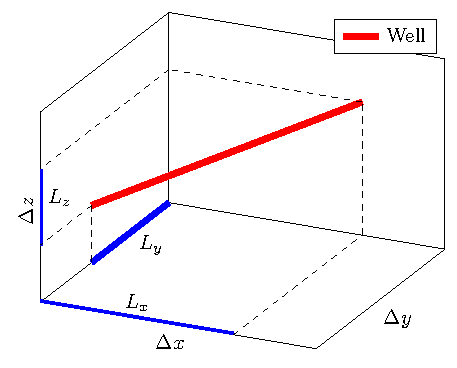
\includegraphics[width=0.80\textwidth]{figures/well_index/well_index.pdf}
	\caption{Well trajectory in a single well block projected 
			 onto the three axes. The projections have lengths $L_x$, $L_y$
			 and $L_z$, and the well block has dimensions $\Delta_x$, $\Delta_y$
			 and $\Delta_z$. This figure is a copy of the one used by Shu in
			 his report \cite{Shu_Paper}}
	\label{fig:well_index}
\end{figure}
%
The well index can now be calculated for slanted wells and
non-square blocks by first calculating the well index for
each direction with
%
\begin{align}
WI_x = \frac{2 \pi \sqrt{k_y k_z} L_x}{\ln \frac{r_{0,x}}{r_w} + s}, \quad WI_y = \frac{2 \pi \sqrt{k_x k_z} L_y}{\ln \frac{r_{0,y}}{r_w} + s}
\quad \text{and} \quad WI_z = \frac{2 \pi \sqrt{k_x k_y} L_z}{\ln \frac{r_{0,z}}{r_w} + s}, 
\end{align}
%
where $k_i$ is the permeability in direction $i$, $r_w$ is the 
wellbore radius, $s$ is the skin factor and
%
\begin{align}
r_{0,x} = 0.28 \frac{ \bigg( \Delta z^2 \left( \frac{k_y}{k_z} \right)^{\frac{1}{2}} +  \Delta y^2 \left( \frac{k_z}{k_y} \right)^{\frac{1}{2}} \bigg)^{\frac{1}{2}} }{ \left( \frac{k_y}{k_z} \right)^{\frac{1}{4}} + \left( \frac{k_z}{k_y} \right)^{\frac{1}{4}} }.
\end{align}
%
The functions $r_{0,y}$ and $r_{0,y}$ are defined in the 
same manner but with the indices $x, y$ and $z$ shifted.
%
At last we take the square root of the sum of the squares
of the directional well indices to get the well index for
the block
%
\begin{align}
WI = \sqrt{WI_x^2 + WI_y^2 + WI_z^2}.
\label{eq:well_index}
\end{align}
%
For the rest of 
this thesis we will simplify the equation by setting $s = 0$, 
i.e., neglecting the skin factor.
%
\section{Computing well trajectory and projection}
% 
In order to compute the well index with \eqref{eq:well_index}
we need not only determine which blocks are penetrated 
by the wells, but also determine the point of entry and
exit. This is done by first using a function called 
\texttt{GetblockEnvelopingPoint()}. This function simply iterates
over all the well blocks of the reservoir and returns the first
block that contains a given point. This is done by checking that
the point is on the correct side (i.e., towards the center of the 
well block) of every face of the block. Using this function on the 
start point will give us the well block that contains the 
starting point as shown in Figure \ref{fig:intersect_block_epsilon}.
%
\begin{figure}[H]
	\centering
	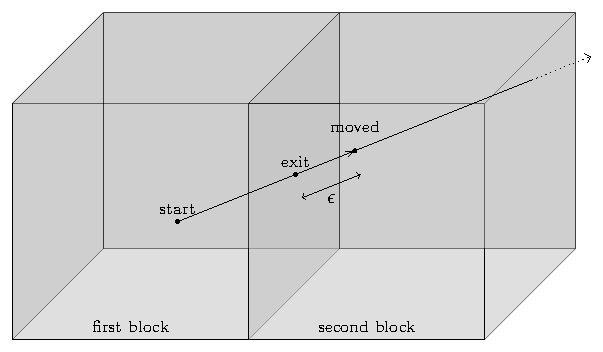
\includegraphics[width=0.80\textwidth]{figures/intersecting_wells/move_point_eps.pdf}
	\caption{Moving a small distance $\epsilon$ along the line segment
			 towards the end of the line segment will ensure that
			 we are completely inside the next block. In the new
			 block we can perform the same steps as we did in the previous block.}
	\label{fig:intersect_block_epsilon}
\end{figure}
%
We then find the intersection point between the well and 
this first block, which we will call the exit point of the well.
Now we have acquired the intersection points for the first well 
block. After this we simply move a sufficiently small 
distance $\epsilon$ from this exit point towards the end of 
the well, and call this new point moved point. With sufficiently
small we mean a small fraction ($\sim \frac{1}{100}$) of the shortest
well side length. Note that this could lead to numerical errors as
we might jump over some blocks if the intersection between the 
well and the block is very short. But if the length of the
intersection is very short, then value of the corresponding well 
index will be very small as well, thus we can neglect it. 
%
Now we can use
the same method as we did for the starting point to get the
intersection points of the second block, and this process can
be repeated until we reach the end of the well.
%
%
Because the corner coordinates of the well block are known, we can compute
the lengths $\Delta_x$, $\Delta_y$ and $\Delta_z$ for each side of the block.
Then we can find the unit vector $\textbf{u}_i$ for the direction of the sides
of the well block. Thus given a well block and its two intersection points,
$\textbf{p}_1$ and $\textbf{p}_2$, the projected well lengths $L_x$, $L_y$ 
and $L_z$ are given by 
%
\begin{align}
L_i = \big\langle (\textbf{p}_2 - \textbf{p}_1), \textbf{u}_i \big\rangle.
\end{align}
%
Supplying the permeabilities $k_i$ and wellbore radius $r_w$ and in the absence
of skin ($s = 0$), we can compute the well index of the block with \eqref{eq:well_index}.
% \clearpage

% -*- root: ../mainThesis.tex -*-
%
\chapter{Implementation}
%
Here we briefly explain the implementations that were
made and the most important part of the code can
be seen in the Appendix. For the full code we refer
to the author's Github repository\cite{Hilmar_git}.
%
\section{Software}
All code was written in Qt 5.5, a cross-platform application and UI 
framework for C++ developed by The Qt Company\cite{QtCompany}.
%
The code makes great use of the Eigen library\cite{Eigen_library} 
which is a template library for linear algebra that includes
matrix and vector classes and algorithms for matrix decompositions.
This is required in the implementation of the inter-well distance
projection for finding the eigenvalue decomposition needed in
\eqref{eq:interwell_s}. The vector class \texttt{Vector3d} of
the Eigen library is also used frequently throughout most
implementations as it contains many useful functions.
%
In order to find the roots of polynomials we make use of the 
RPOLY library \cite{Rpoly}, which is an implementation of the 
Jenkins-Traub algorithm\cite{Jenkins_traub}. This is needed for
solving the sixth degree equation \eqref{eq:six_degree_poly} 
which is the most important part of the inter-well distance 
projection.
%
%
\section{Well length constraint projection}
%
The function \texttt{well\_length\_projection\_eigen()}, takes
the initial coordinates of the heel and toe of a well, and by
calculating the distance between them it determines which of the 
solutions \eqref{eq:solution_min_triv} -- \eqref{eq:wl_formula_last}
it should return.  
%
%
\section{Inter-well distance constraint projection}
%
In the function \texttt{interwell\_constraint\_projection\_eigen()}
which was implemented we take the initial coordinates of two
wells and a distance $d$ as input. Then we try to find solutions by 
moving as few points as possible. First we try to move only two
points by using \texttt{well\_length\_projection\_eigen()}.
If some two-point solution is feasible for the complete
problem we return the best one. If no two-point solution is
found we try the three-point solutions. This is done by
building $A$ and $b$ according to \eqref{eq:A_b_three_points},
and then running \texttt{kkt\_eq\_solutions\_eigen($A,b$)} which
returns all candidate solutions of \eqref{eq:interwell_matrix}.
If one or more feasible solutions are found we pick the best one.
If no solution has been found yet we must have a four-point
solution. We build $A$ and $b$ according to \eqref{eq:A_b_three_points}
and pick the best solution returned by 
\texttt{kkt\_eq\_solutions\_eigen($A,b$)}.
%
\section{Alternating projections}
%
Now that both well length projection and inter-well distance
projection are available, the method of alternating projections
is simply done by running one projection after the other inside
a while loop until the well positions are feasible. Note that
we can also change the order of the projections, which might
impact the solution. In our implementation the inter-well
distance projection was done first.
%
\section{Well index calculation and intersecting blocks}
%
In order to compute the well indices for the well blocks
of a reservoir, we first need to determine which blocks
are penetrated by a well and what the entry and exit points
are. If these two steps are handled, then computing the well
index for each block is done by computing the well block
projections as shown in Figure \ref{fig:well_index} and then
supplying the block dimensions and permeabilities and using
\eqref{eq:well_index}. Here we describe the algorithm
used to find the well blocks which are intersected by a well
and in which points the intersections occur. Well blocks will
only be referred to as blocks.
%
Assume that \texttt{GetblockEnvelopingPoint($p$)} returns a block 
that contains the point $p$. Assume also that \texttt{FindIntersectionPoints}(block, line)
calculates the two intersection points 
between a line segment and a block.\\
%
A list of intersected blocks and their entry and exit points are created
and returned at the end of the algorithm.
%
\begin{algorithm}
\caption{Input: reservoir(blocks), line(start point, end point) }\label{alg:block_intersection}
\begin{algorithmic}[1]
\Procedure{Find intersected blocks}{}
\State first block $\gets$ \texttt{GetblockEnvelopingPoint}(start point)
\State last block $\gets$ \texttt{GetblockEnvelopingPoint}(end point)
\State Set current block = first block
\State 
\While {current block $!=$ last block}
	\State intersection points $\gets$ \texttt{FindIntersectionPoints}(current block, line)
	\State add intersection points to list
	\State add current block to list
	\State
	\State new point $\gets$ Move small distance out of current block in direction of \hspace{10mm} .\hspace{10mm} end point
	\State 
	\State current block $\gets$ \texttt{GetblockEnvelopingPoint}(new point)
	\State 
\EndWhile

\State Add last block to list
\State Return lists

\EndProcedure
\end{algorithmic}
\end{algorithm}
 \clearpage

% CHAPTER 5: IMPLEMENTATION 1 + TESTING: 
% SOLVE CONSTRAINT HANDLING PROBLEM FOR SIMPLE CASE
% Sub problem 1: WELL LENGTH CONSTRAINT
% Sub problem 2: INTER WELL DISTANCE CONSTRAINT
% Sub problem 3: WELL DOMAIN
% CHAPTER 6: IMPLEMENTATION 2 + TESTING: 
% SOLVE SIMBLE WELL PLACEMENT OPTIMIZATION CASE USING
% DEVELOPED CONSTRAINT HANDLING TECHNIQUE + WELL INDEX 
% CALCULATION
% -*- root: ../mainThesis.tex -*-
\chapter{Results and numerical tests} 
In this chapter we present the results of the implementations
of the well distance projection and the inter-well distance 
projection and the alternating projection method applied to the
joint problem. We also include numerical results from the computations
of well indices and compare them to the results found using 
the reservoir simulator RMS. Figures are also supplied whenever
possible. 
%
\section{Well constraint projections}
%
For all projections in this section we set the well length constraint 
(i.e., shortest and longest wells allowed) and inter-well distance 
constraint (i.e., the minimum distance required to be between all 
pairs of wells) parameters to the following values:
%
\begin{align}
L_{\min} &= 5,  \\
L_{\max} &= 10, \\
d &= 4.
\label{eq:constraint_parameters}
\end{align}
%
This means that in the final configuration all wells must have a 
length between 5 and 10, and no two wells are allowed to be 
closer than a distance 4 to each other.
%
The well length projection was tested on a single well and 
simultaneously on a set of five wells. the inter-well distance 
projection was tested on two wells and then as an alternating projection
on five wells. Both projections were then applied alternatingly on one
set of two wells and one set of five wells until a feasible solution was 
reached.
%
\subsection{Well length projection}
%
%
\paragraph{Well length constraint on a single well}
%
First consider the well with endpoints $(-\frac{1}{2},0,\frac{1}{2})$
and $(\frac{1}{2},0,\frac{1}{2})$. This well has length 2 and its length
is increased as shown in Figure \ref{fig:trivial_min}.
%
\begin{figure}[H]
	\centering
	\begin{subfigure}{0.44\textwidth}
		\centering
		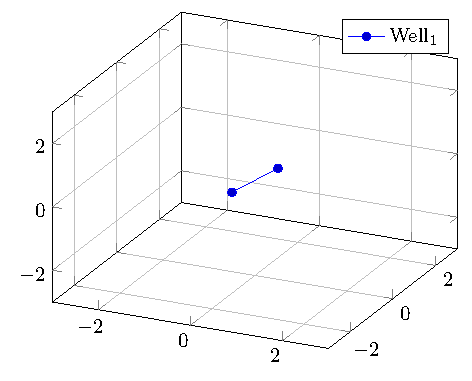
\includegraphics[width=1\textwidth]{figures/trivial_projections/trivial_initial.pdf}
		\caption{Initial well. The well has length 2 and violates the well length constraint
				  because it is too short.}
		\label{fig:trivial_min_a}
	\end{subfigure}\hfill
	\hspace{.05\linewidth}
	\begin{subfigure}{0.44\textwidth}
		\centering
		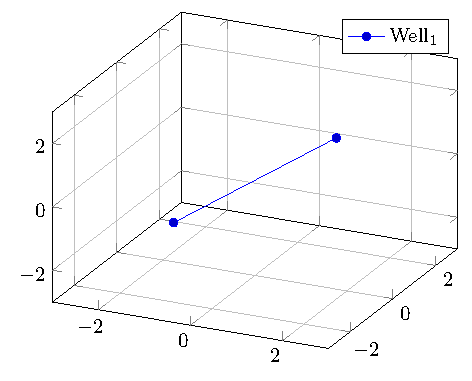
\includegraphics[width=1\textwidth]{figures/trivial_projections/trivial_min.pdf}
		\caption{The well has been projected to satisfy the well length length constraint.
				  The projected well has length 5 which is equal to $L_{\min}$.}
		\label{fig:trivial_min_b}
	\end{subfigure}
	\caption{The well on the left that violates the well length constraint
			 has been projected to a feasible solution on the right.}
	\label{fig:trivial_min}
\end{figure}
%
%
Now consider the well with endpoints $(-5,-5,-5)$,
$(5,5,5)$. This well has length $10\sqrt{3}$ and its length
is decreased as shown in Figure \ref{fig:trivial_max}.
%
\begin{figure}[H]
	\centering
	\begin{subfigure}{0.44\textwidth}
		\centering
		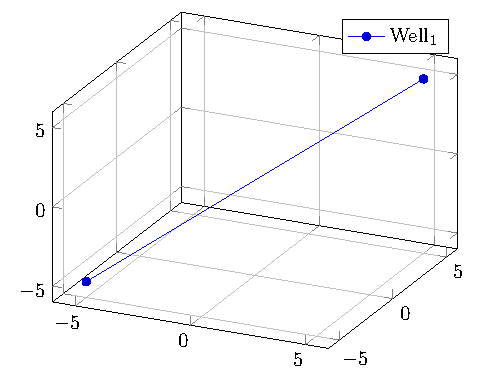
\includegraphics[width=1\textwidth]{figures/trivial_projections/trivial_initial_max.pdf}
		\caption{Initial well. The well has length $10\sqrt{3}$ and violates the well length constraint
				  because it is too long.}
	\end{subfigure}\hfill
	\hspace{.05\linewidth}
	\begin{subfigure}{0.44\textwidth}
		\centering
		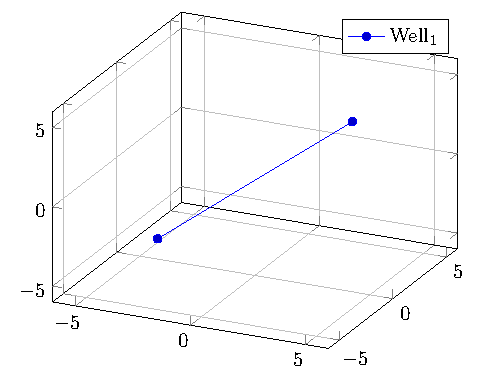
\includegraphics[width=1\textwidth]{figures/trivial_projections/trivial_max.pdf}
		\caption{The well has been projected to satisfy the well length length constraint.
				  The projected well has length 10 which is equal to $L_{\max}$.}
	\end{subfigure}
	\caption{The well on the left that violates the well length constraint
			 has been projected to a feasible solution on the right.}
	\label{fig:trivial_max}
\end{figure}
%
Lastly five wells were were created as shown in Figure \ref{fig:initial_5_well}.
%
\begin{figure}[H]
	\centering
	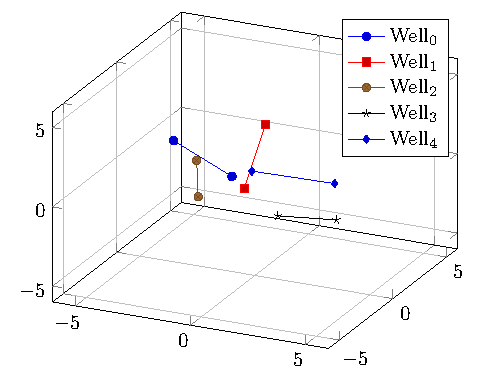
\includegraphics[width=0.70\textwidth]{figures/interwell_distance/five_wells.pdf}
	\caption{Initial positions of five wells. Both the well distance constraint and the
											  inter-well distance constraint are violated
											  by one or more wells.}
	\label{fig:initial_5_well}
\end{figure}
%
Note that since the well lenghts are independent from
each other the well lenght projection of multiple wells is
eqivalent to sequential projection of single wells.
In Figure \ref{fig:initial_5_well_length} we can see the
five well length projections.
%
\begin{figure}[H]
	\centering
	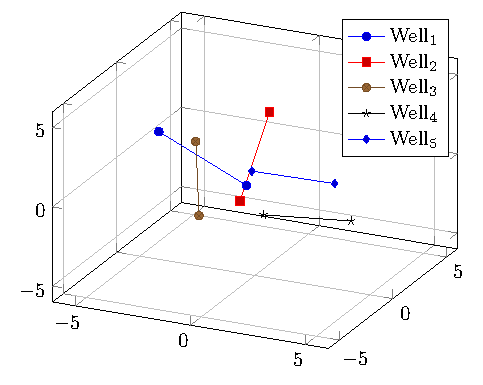
\includegraphics[width=0.70\textwidth]{figures/well_length/well_length_moved.pdf}
	\caption{Well length projection on five wells. Five wells have been moved so that the well
										length constraint is satisfied for all wells.
										The inter-well distance constraint however is
										not satisfied.}
	\label{fig:initial_5_well_length}
\end{figure}
%
\subsection{Inter-well distance projection}
%
The inter-well distance projection was first tested on two wells,
$\text{Well}_1$ and $\text{Well}_2$, with initial coordinates 
%
\begin{align*}
\text{Well}_1 = \left( (-1,0,0), (0,1,0) \right) \quad \text{and} \quad  \text{Well}_2 = \left( (0,-1,0), (1,0,0) \right).
\end{align*}
%
Note that the wells in this case are parallel and, as
mentioned in Section 3.2.1, there is no unique shortest 
distance line between the two wells. Still the numerical
solution is found and the resulting four-point solution 
can be seen in Figure \ref{fig:trivial_interwell_1}.
%
\begin{figure}[H]
	\centering
	\begin{subfigure}{0.44\textwidth}
		\centering
		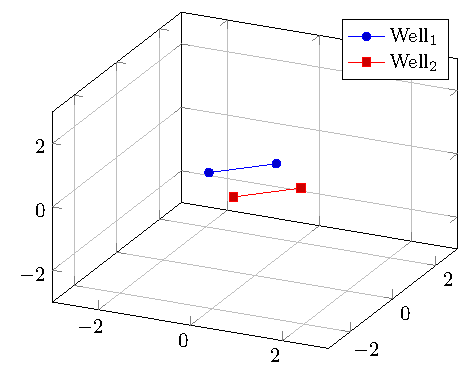
\includegraphics[width=1\textwidth]{figures/interwell_distance_two_wells/initial.pdf}
		\caption{Initial wells. The shortest distance between the wells is $\sqrt{2}$ which is
								 less than $d=4$, and thus the inter-well distance constraint is
								 violated.}
	\end{subfigure}\hfill
	\hspace{.05\linewidth}
	\begin{subfigure}{0.44\textwidth}
		\centering
		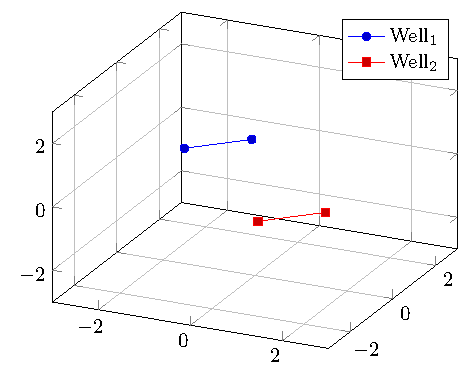
\includegraphics[width=1\textwidth]{figures/interwell_distance_two_wells/initial_moved.pdf}
		\caption{The wells have been moved so the the shortest distance between them is 4.}
	\end{subfigure}
	\caption{The wells initial positions don't satisfy the inter-well distance constraint. The wells
						are moved so that the shortest distance between them is exactly equal to $d = 4$.}
	\label{fig:trivial_interwell_1}
\end{figure}
%
The inter-well distance projection was then tested on two 
wells $\text{Well}_3$ and $\text{Well}_4$, with initial
coordinates 
%
\begin{align*}
\text{Well}_3 = \left( (-2,-2,0), (-2,2,0) \right) \quad \text{and} \quad  \text{Well}_4 = \left( (0,0,0), (3,0,0) \right).
\end{align*}
%
The point to the right on $\text{Well}_4$ is exactly a distance 4 away from $\text{Well}_3$,
but clearly the points of $\text{Well}_3$ will be moved to the left, so we expect the right
point on $\text{Well}_4$ to remain static. Indeed the projection, which is shown in Figure
\ref{fig:trivial_interwell_2} only moves 3 points, and we have a three-point solution.
%
\begin{figure}[H]
	\centering
	\begin{subfigure}{0.44\textwidth}
		\centering
		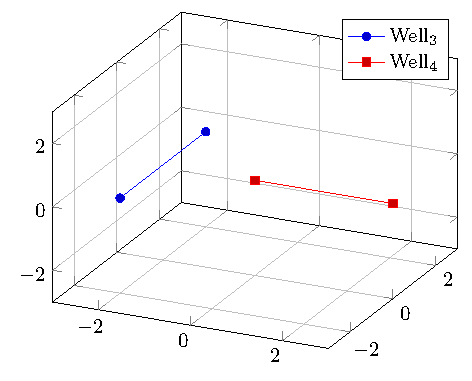
\includegraphics[width=1\textwidth]{figures/interwell_distance_two_wells/initial_2.pdf}
		\caption{Initial wells. The shortest distance between the wells is 1 which is
								 less than $d=4$, and thus the inter-well distance constraint is
								 violated.}
	\end{subfigure}%\hfill
	\hspace{.05\linewidth}
	\begin{subfigure}{0.44\textwidth}
		\centering
		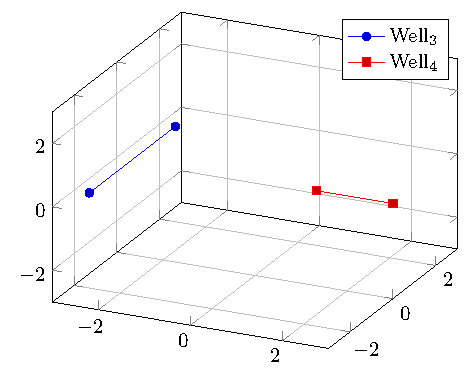
\includegraphics[width=1\textwidth]{figures/interwell_distance_two_wells/initial_2_moved.pdf}
		\caption{The wells have been moved so the the shortest distance between them is 4.}
	\end{subfigure}%
	\caption{The wells initial positions don't satisfy the inter-well distance constraint. The wells
						are moved so that the shortest distance between them is exactly equal to $d = 4$.
						The point to the right on $\text{Well}_4$ is not moved at all, which means this
						is a three-point solution as discussed in Chapter 3.}
	\label{fig:trivial_interwell_2}
\end{figure}
%
We refer to Chapter 8 for discussion on a single projection that failed.
%
\subsection{Alternating projections to joint problem}
%
We start with alternating projections on two wells with initial
coordinates $\left( (-2,-2,0), (-2,2,0) \right)$ and $\left( (0,0,0), (3,0,0) \right)$
as seen in Figure \ref{fig:alternate_two_a}. The resulting position in Figure 
\ref{fig:alternate_two_b} took 8 alternating iterations to be reached. 

%
\begin{figure}[H]
	\centering
	\begin{subfigure}{0.44\textwidth}
		\centering
		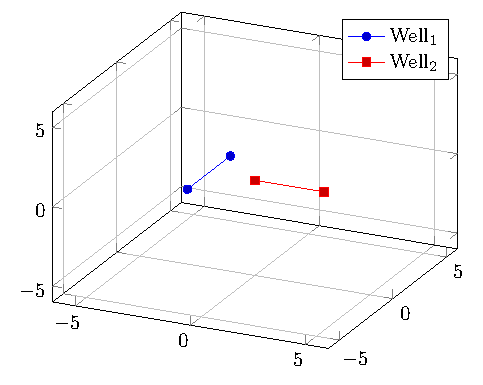
\includegraphics[width=1\textwidth]{figures/both_projections/two_wells_initial.pdf}
		\caption{Initial wells. The shortest distance between the wells is 1 which is
								 less than $d=4$, and thus the inter-well distance constraint is
								 violated.}
		\label{fig:alternate_two_a}
	\end{subfigure}%\hfill
	\hspace{.05\linewidth}
	\begin{subfigure}{0.44\textwidth}
		\centering
		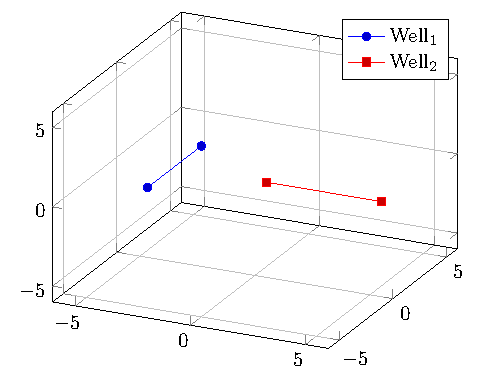
\includegraphics[width=1\textwidth]{figures/both_projections/two_wells_moved.pdf}
		\caption{The wells have been moved so the the shortest distance between them is 4 and
				 the lengths of the wells have been adjusted.}
		\label{fig:alternate_two_b}
	\end{subfigure}%
	\caption{The wells initial positions don't satisfy the inter-well distance constraint. The wells
						are moved so that the shortest distance between them is exactly equal to $d = 4$.
						The point to the right on $\text{Well}_4$ is not moved at all, which means this
						is a three-point solution as discussed in Chapter 3.}
	\label{fig:alternate_two}
\end{figure}
%
Actually the constraints are never fully satisfied in this case because
the projections work against each other. We have implemented a tolerance
for accepting a position as feasible, but in this case we can get arbitrarily
close to a feasible solution given enough iterations.
%

Now the five wells seen in Figure \ref{fig:initial_5_well} 
are projected using alternating projections. Theoretically 
there is no guarantee that any of the projections will
converge.
%
First we use the inter-well distance projection on pairs
of wells until a feasible solution is reached. After iterating
four times over all pairs of wells the solution in Figure
\ref{fig:initial_5_well_distance} was found.
%
\begin{figure}[H]
	\centering
	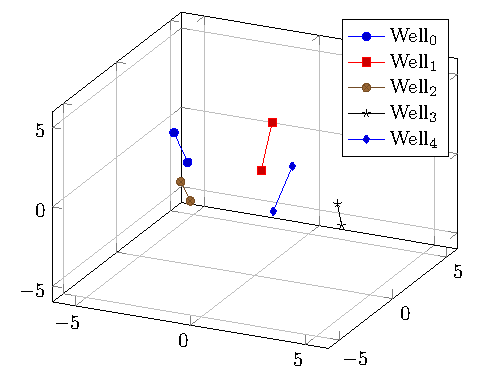
\includegraphics[width=0.70\textwidth]{figures/interwell_distance/five_wells_moved.pdf}
	\caption{Inter-well distance projection on five wells. By running inter-well projection on 
											 wells pairwise, the five wells have been moved so 
											 that the inter-well distance constraint is satisfied 
											 for all pairs of wells. The Solution took four steps of 
											 iterating over all pairs. The well length constraint 
											 is not satisfied for any of the wells because they
											 are all too short. This is not surprising because the inter-well
											 distance projection can only shorten the length of a well.}
	\label{fig:initial_5_well_distance}
\end{figure}
%
%
Finally both projections were done alternatingly until
the five wells satisfied both constraints. The final
positions of the wells, which can be seen in Figure 
\ref{fig:initial_5_both}, was found after six iterations
of each projection. Again the solution is not feasible
but the error is sufficiently small to stop the iterations.
%
\begin{figure}[H]
	\centering
	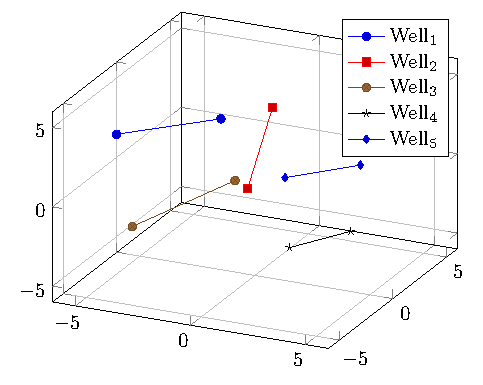
\includegraphics[width=0.70\textwidth]{figures/both_projections/both_projections.pdf}
	\caption{Alternating well length- and inter-well distance projection. By alternating between
											well length projection and inter-well distance projection
											the wells have been moved so that the well length constraint
											is satisfied for all wells and the inter-well distance constraint
											is satisfied for all pairs of wells. The solution took six 
											steps of alternating projections.}
	\label{fig:initial_5_both}
\end{figure}
%
%
\section{Well index calculation}
%
We use a reservoir containing $60 \times 60$ well blocks with
dimensions $\Delta_x = \Delta_y = \Delta_z = 24$ and varying 
permeabilities. We ran the intersecting well blocks and well 
index calculation algorithms on a well with wellbore radius
$r_w = \frac{0.1905}{2}$,
which runs from the middle of the block located in the bottom
left corner and straight to the block in the bottom right corner
as indicated by Figure \ref{fig:well_intersection}.
%
\begin{figure}[H]
	\centering
	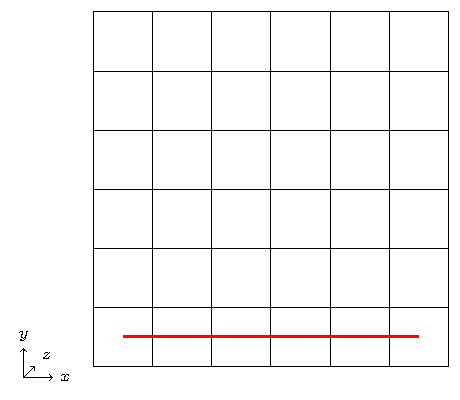
\includegraphics[width=0.40\textwidth]{figures/well_index/well_intersection.pdf}
	\caption{Well that goes from block 0 in the bottom left corner and ends up
	in block 59 in the bottom right corner. For illustration purposes the figure has been edited and every 
	square actually contains 10 $\times$ 10 blocks}
	\label{fig:well_intersection}
\end{figure}
%
The calculated well indices from the first few well
blocks of our implementation and the results obtained 
from RMS can be seen in Table \ref{tab:well_indexes}. 
%
\begin{center}
	\captionof{table}{Computed well indices compared to the well indices calculated by RMS}
	\begin{tabular}[h]{ccc}
	Block number & Well index (Our algorithm) & Well index (RMS) \\
	\hline
	\hline
	0 & 0.213273 & 0.21327 \\
	1 & 0.328879 & 0.32888 \\
	2 & 0.328879 & 0.32888 \\ 
	3 & 0.501907 & 0.50191 \\
	4 & 0.471228 & 0.47123 \\
	5 & 0.593556 & 0.59356 \\
	6 & 0.924533 & 0.92453 \\
	7 & 1.287440 & 1.28744 \\
	8 & 0.905511 & 0.90551
	\label{tab:well_indexes}
	\end{tabular}
\end{center}
%
%
 \clearpage

% CHAPTER 7: SUMMARY
% -*- root: ../mainThesis.tex -*-
\chapter{Summary and discussion}
%
We summarize the results of the projection methods
and the well index calculator and comment on the
main points of them. 

The main goal of the thesis was the solution of two sub-problems 
occurring during the tackling of well-placement optimization, namely 
handling of well constraints and well index calculations. These
are important because they reflect physical properties of the 
reservoir and are essential for a reliable and practical way
of solving the overall well placement problem. 
%
\section{Projection to feasible space}
%
The first problem we discussed was the handling of 
well-placement constraints. Here we introduced and 
implemented a method based on alternating projections, 
where one of the projections could be solved analytically, 
while the other projection had to be solved numerically.

The alternating projection method for satisfaction
of inter-well distance and well distance constraint
was implemented. The well distance constraint was
solved and the analytical solutions were derived
and implemented. 

The main issue was the derivation
of an accurate method for the projection on the 
inter-well distance constraint. The idea of splitting
up the problem into $k$-point solutions leads to
different cases. The main sub-case is finding the
roots of the sixth degree polynomial in \eqref{eq:six_degree_poly},
which can be done efficiently with arbitrarily high
precision. The implemented version preformed well
overall and managed to even solve cases where one
would expect numerical issues, such as when
all wells are along the same line. However, the 
implementation was not able to solve one case 
with parallel line segments which is presented 
in Chapter 8. The reason for this is unknown.
%
\section{Well index calculation}
%
The goal for the well index calculator was to
implement an alternative method capable of 
dealing with deviated and slanted wells.
%%%%%%%%%%%%%%%%%%
The method works by taking weighted means of the well 
indices one would obtain for centered wells parallel to 
the block axes, with weights depending on the projections 
of the well on these axes. To do this we require  
computations of entry and exit points of each of the
blocks penetrated by the well.

The implemented algorithm for finding well
indices compared well to industry standards
for well index calculations.
%
 \clearpage

% CHAPTER 7: FURTHER WORK
% -*- root: ../mainThesis.tex -*-
\chapter{Further work}
%
There were several things that we were not able
to do due to either lack of time or simply because 
we were not able to solve the problem. Here we
list the most important things and provide some
information for further work.
%
\section{FieldOpt integration}
%
All functions need to be slightly adjusted so they
can be included into FieldOpt and integrated for
the optimization problem. The main reason is that
FieldOpt uses its own well and coordinate classes,
so we have to adjust the input and output format of
our code.
%
\section{Well length constraint projection}
%
The well length constraint projection only
handles wells that consist of a single straight line 
segment. There is no obvious extension of the 
current solution for non-straight wells. In the 
case of wells consisting of several connected 
straight lines there is an extension of our current algorithm
which is to only move the heel and toe along
the trajectory of the initial well. Extending
the lines beyond the initial lenght of the
well doesn't have a unique solution, since all
directions are feasible. This works 
perfectly well for wells consisting of multiple
line segments as long as the angles between the line 
segments are less than $45^\circ$.
%
\section{Inter-well distance constraint projection}
%
Note first that we were able to find one
case where our algorithm was not able to
solve the inter-well distance problem. This
is a simple case with two parallel shifted
line segments as shown in Figure \ref{fig:inter_well}.
%
\begin{figure}[H]
	\centering
	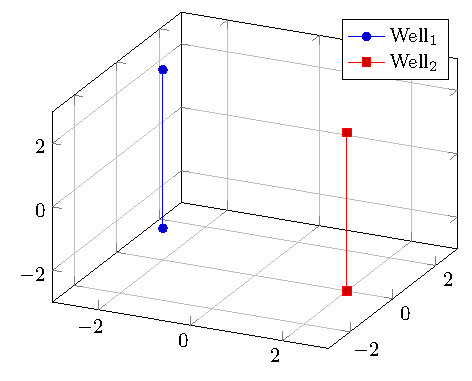
\includegraphics[width=0.80\textwidth]{figures/further_work/inter_well_distance.pdf}
	\caption{Well length projection on five wells. Five wells have been moved so that the well
										length constraint is satisfied for all wells.
										The inter-well distance constraint, however, is
										not satisfied.}
	\label{fig:inter_well}
\end{figure}
%
Several very similar cases were tried and
solutions were found for all of them. We
did not have time to resolve the problem
for this exact case, but we believe that 
the problem is due to numerical errors.
%
Every time we solve equation \eqref{eq:interwell_s}
there might be numerical issues when
computing the eigendecomposition of $A$.
Mathematically speaking there are no problems
involved in solving \eqref{eq:interwell_s}, but 
some care should be taken in these computations
to guarantee that a solution is found.
%
%
\section{Alternating projections}
%
The convergence of the alternating projection of well length
projection and inter-well distance projection was not proven.
From the results obtained for several wells it is reasonable 
to expect that the alternating projection will always converge.
The inter-well distance projection always moves pairs of wells
away from the average coordinate of their endpoints, whilst the
well length projection always leaves the average of the heel
and toe of a well unchanged. Because there was no spatial
restriction in our work, we hypothesize that the inter-well
distance projection will simply move points away from the
average of all the points until a solution is found.
Possible alternatives to the method of alternating projections, 
which might be worthwhile looking into, could be averaged 
projections \cite{Lewis_Luke_Malick_2} or Dykstra's projection
algorithm.
% \clearpage

\appendix
% -*- root: ../mainThesis.tex -*-
%
\chapter{Code}

\section{Code for well constraint projection}
%
\texttt{well\_length\_projection\_eigen()}
\lstinputlisting[language=c++]{code/well_length_projection.cpp}
%
\section{Code inter-well distance projection}
%
\texttt{interwell\_constraint\_projection\_eigen()}
\lstinputlisting[language=c++]{code/interwell_constraint_projection_eigen.cpp}
%
\texttt{kkt\_eq\_solutions\_eigen()}
\lstinputlisting[language=c++]{code/solve_kkt_equation.cpp}
%
% APPENDIX A: CODE FOR CONSTRAINT HANDLING

% APPENDIX B: CODE FOR WELL INDEX CALCULATION





% ==========================================================
% REFERENCES
\bibliographystyle{IEEEtran}
\bibliography{/home/cutie/Dropbox/SharedFieldOptDev15/files_HM/Thesis/bibtex_references/references}
\clearpage

\end{document}\grid